\documentclass[a4paper,12pt]{article}
%\documentclass{Configuration_Files/Template}

%------------------------------------------------------------------------------
%	REQUIRED PACKAGES AND  CONFIGURATIONS
%------------------------------------------------------------------------------

% CONFIGURATIONS
\usepackage{parskip} % For paragraph layout
\usepackage{setspace} % For using single or double spacing
\usepackage{emptypage} % To insert empty pages
\usepackage{multicol} % To write in multiple columns (executive summary)
\setlength\columnsep{15pt} % Column separation in executive summary
\setlength\parindent{0pt} % Indentation
\raggedbottom  

% PACKAGES FOR TITLES
\usepackage{titlesec}
% \titlespacing{\section}{left spacing}{before spacing}{after spacing}
\titlespacing{\section}{0pt}{3.3ex}{2ex}
\titlespacing{\subsection}{0pt}{3.3ex}{1.65ex}
\titlespacing{\subsubsection}{0pt}{3.3ex}{1ex}
\usepackage{color}

% PACKAGES FOR LANGUAGE AND FONT
\usepackage[english]{babel} % The document is in English  
\usepackage[utf8]{inputenc} % UTF8 encoding
\usepackage[T1]{fontenc} % Font encoding
\usepackage[11pt]{moresize} % Big fonts

% PACKAGES FOR IMAGES
\usepackage{graphicx}
\usepackage{transparent} % Enables transparent images
\usepackage{eso-pic} % For the background picture on the title 
\usepackage{rotating}
\usepackage{subfig} % Numbered and caption subfigures using \subfloat.
\usepackage{tikz} % A package for high-quality hand-made figures.
\usetikzlibrary{}
\graphicspath{{./Images/}} % Directory of the images
\usepackage{caption} % Coloured captions
\usepackage{amsthm,thmtools,xcolor} % Coloured "Theorem"
\usepackage{float}

% STANDARD MATH PACKAGES
\usepackage{amsmath}
\usepackage{amsthm}
\usepackage{amssymb}
\usepackage{amsfonts}
\usepackage{bm}
\usepackage[overload]{empheq} % For braced-style systems of equations.
\usepackage{fix-cm} % To override original LaTeX restrictions on sizes

% PACKAGES FOR TABLES
\usepackage{tabularx}
\usepackage{longtable} % Tables that can span several pages
\usepackage{colortbl}
\usepackage{multicol}
\newcolumntype{C}[1]{>{\centering\arraybackslash}m{#1}} % Centered column type
\setlength\columnsep{15pt}

% PACKAGES FOR ALGORITHMS (PSEUDO-CODE)
\usepackage{algorithm}
\usepackage{algorithmic}

% PACKAGES FOR REFERENCES & BIBLIOGRAPHY
\usepackage[colorlinks=true,linkcolor=black,anchorcolor=black,citecolor=black,filecolor=black,menucolor=black,runcolor=black,urlcolor=black]{hyperref} % Adds clickable links at references
\usepackage{cleveref}
\usepackage[square, numbers, sort&compress]{natbib} % Square brackets, citing references with numbers, citations sorted by appearance in the text and compressed
\bibliographystyle{abbrvnat} % You may use a different style adapted to your field

% OTHER PACKAGES
\usepackage{pdfpages} % To include a pdf file
\usepackage{afterpage}
\usepackage{lipsum} % DUMMY PACKAGE
\usepackage{fancyhdr} % For the headers
\fancyhf{}

%----------------------------------------------------------------------------
%	NEW COMMANDS DEFINED
%----------------------------------------------------------------------------

% EXAMPLES OF NEW COMMANDS
\newcommand{\bea}{\begin{eqnarray}} % Shortcut for equation arrays
\newcommand{\eea}{\end{eqnarray}}
\newcommand{\e}[1]{\times 10^{#1}}  % Powers of 10 notation

%----------------------------------------------------------------------------
%	ADD YOUR PACKAGES (be careful of package interaction)
%----------------------------------------------------------------------------

\usepackage{geometry}
\usepackage{tabularx}
\usepackage{booktabs,xltabular}

%----------------------------------------------------------------------------
%	ADD YOUR DEFINITIONS AND COMMANDS (be careful of existing commands)
%----------------------------------------------------------------------------

% Set uniform margins
\geometry{
  left=0.8in,
  right=0.8in,
  top=1in,
  bottom=1in,
  includehead,
  includefoot
}

\begin{document}
\title{Students\&Companies Design Document} % Title Page
\author{Alessandro Salvatore, Erdal Yalçın, Leonardo Ratti}
\date{Academic Year: 2024-25}
\maketitle


\newpage
\tableofcontents
\section{Introduction}
\subsection{Purpose}
This document contains the design description of the Students\&Company system. It includes
the architectural design, the user interface design and the descrpition of the operations
that the system will perform. It also show how the requirements and use cases detailed
in the RASD document are satisfied by the design of the system. \\ \newline 
This document is intended to be read by the developers of the system, the testers and the
project managers. It is also intended to be used as a reference for the future maintenance
of the system.
\subsection{Scope}
The Students\&Company system is a web application that allows companies to advertise internship opportunities
for university students. A recommendation system is used for enhancing the matching possibilities between the two parties.
The system provides also suggestions for students and companies to increase their chances to get matched by the recommendation system. \\ \newline
A more detailed description of the system can be found in the RASD document, whilist in
this document is provided a detailed description of the design of the system to implement
the requirements and use cases described in the RASD document.
\subsubsection{Definitions}
    \begin{itemize}
        \item \textbf{User}: with User we refer to an active individual that can be either a Student, a Comapny or a University.
        \item \textbf{Advertise}: An Internship is advertised only if it has been posted and its application deadline is not yet expired.
        \item \textbf{Recommendation}: It's a platform feature that starts a matching between a company and a student. If both parties accept the recommendation, the student is taken for the selection process
        \item \textbf{Applying}: a student applies for an internship if he/she manually searches for it and applies for it and the internship was not recommended to him/her.
        \item \textbf{Accepting}: The act of students or companies, who got recommended to each other, to confirm their interest.
        \item \textbf{Contact}: The mutual acceptance of recommendation between student and company on the same internship.
        \item \textbf{Selection}: It's the process that starts after the expiration date of applying for the internship. The company interviews every accepted student and picks the best one(s) for their needs.
        \item \textbf{Selected student}: He is the student who has been chosen for the internship by the company.
        \item \textbf{Candidate}: he is a Student that has passed to the selection phase of an internship.
        \item \textbf{Feedback}: Consists of two separate moments.
        The first round of feedback is when the users likes/dislikes the recommendation given by the system. The second type of feedback is submitted after the end of the internship, where students and companies rate the experience through a 5 star review form.
        \item \textbf{Comment}: Is anything written in the dedicated Comments section. Serves the student or the company currently engaged, to highlight something about the experience with each other. If that's a complaint from either, the University of the student will manage the situation.
        \item \textbf{Complaint}: It's a specific type of Observation, where the University of the student can manage the situation between the parties.
        \item \textbf{Observation}: It's a type of comment that is not a complaint. It could just report some good or neutral facts about the experience.
    \end{itemize}
\subsubsection{Acronyms}
    \begin{itemize}
        \item S\&C: "Students\&Companies", the name of the platform
    \end{itemize}
\subsubsection{Abbreviations}
    \begin{itemize}
        \item \textbf{Wn}: n-th World Phenomena
        \item \textbf{Sn}: n-th Shared Phenomena
        \item \textbf{Gn}: n-th Goal
        \item \textbf{Dn}: n-th Domain Assumption
        \item \textbf{Rn}: n-th Requirement
        \item \textbf{Cn}: n-th Component
    \end{itemize}
\subsection{Revision History}
\noindent
\begin{tabularx}{\textwidth}{llX}
    \toprule
    Revised on & Version & Description \\
    \midrule
    07-Jan-2025 & 1.0 & Initial Release of the document \\
    \bottomrule
\end{tabularx}
\subsection{Reference Documents}
    \begin{itemize}
        \item The specification document of the project: \textbf{Assignment RDD AY 2024-2025}
        \item The \textbf{RASD} document of the project

    \end{itemize}
\subsection{Document Structure}
The document is divided into 6 sections:

\begin{itemize}
    \item \textbf{Introduction}: provides a brief description of the purpose and the scope of the system. Moreover, it contains the definitions, acronyms, and abbreviations used in the document and the reference documents.
    
    \item \textbf{Architectural Design}: this section provides a description of the architecture of the system, including the components and the interfaces between them. It also includes the runtime view of the most important operations of the system, the deployment view, and the architectural styles and patterns used in the system.
    
    \item \textbf{User Interface Design}: includes the mockups of the user interface of the system.
    
    \item \textbf{Requirements Traceability}: this section shows how the requirements described in the RASD document are satisfied by the design of the system.
    
    \item \textbf{Implementation, Integration and Test Plan}: this includes the step-by-step plan for the implementation and testing of the system.
    
    \item \textbf{Effort Spent}: this section highlights the effort spent by each member of the group to redact this document.
\end{itemize}

\section{Overall Description}
\subsection{Overview: High-level Components and Interaction}
The following diagram is designed to clearly demonstrate the high-level components required by the system and the relationships between them. 

 The Presentation Layer interacts directly with users and is responsible for managing the front-end side. This layer provides the user interface and collaborates with the Load Balancer and Web Server to optimize system performance and functionality. User interactions within the interface are forwarded from the Presentation Layer to the back-end, enabling additional processing and functionality. Furthermore, to enhance the system’s security and mitigate potential threats from external networks, a Firewall component is incorporated into the architecture. The Business Logic Layer processes incoming requests from the Presentation Layer and facilitates access to the core system functionalities, such as internship applications and recommendation mechanisms, through the use of APIs and Services. In summary, the Business Logic Layer, which houses the Application Server designed in accordance with RESTful standards, ensures the seamless transfer of operations to the Data Layer, thus ensuring the system operates in an efficient, secure, and effective manner.
\begin{figure}[H]
\centering
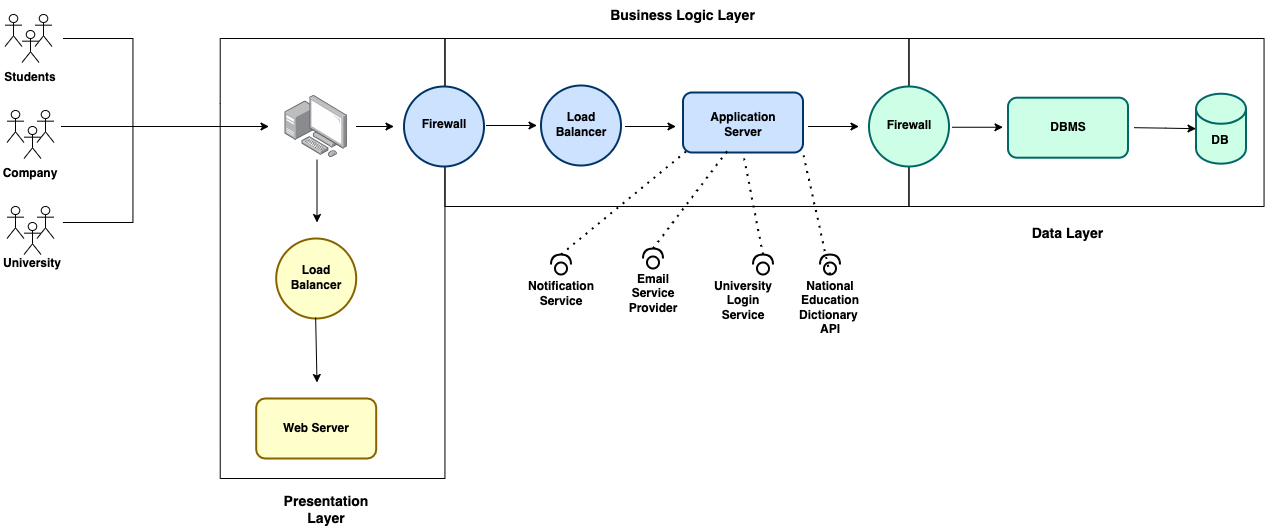
\includegraphics[scale = 0.40]{DD_figures/SingleDiagrams/overviewDiagram.png}
\end{figure}
\subsection{Component View}
In this section we show the components and their relationships. The following
sections will explain the interaction between interfaces and details on each method of interfaces.
\begin{figure}[H]
\centering
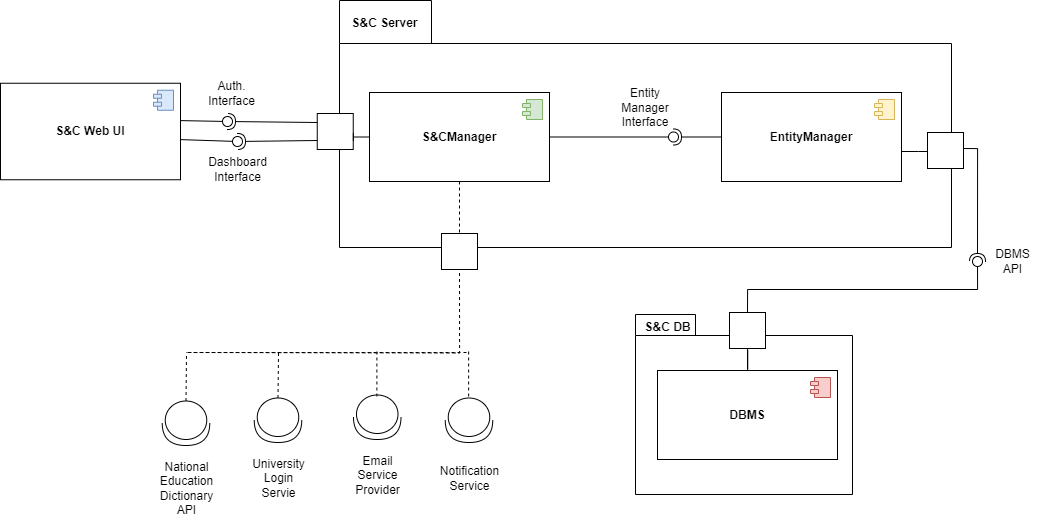
\includegraphics[scale = 0.50]{DD_figures/GeneralComponentDiagram.drawio.png}\\
\caption{Component Diagram of the Student\&Companies System}
\end{figure}

\subsubsection{DB Manager}
This component is responsible for communication with a Database Management System (DBMS).
It follows the Adapter design pattern, allowing other components to interact with the DBMS
without needing to write any SQL code themselves.
\subsubsection{S\&C-SP}
The S\&CSP subsystem implements S\&C's logic. It provides all the system's features, including the recommendation system.
\begin{sidewaysfigure}% Use sidewaysfigure instead of figure
\centering
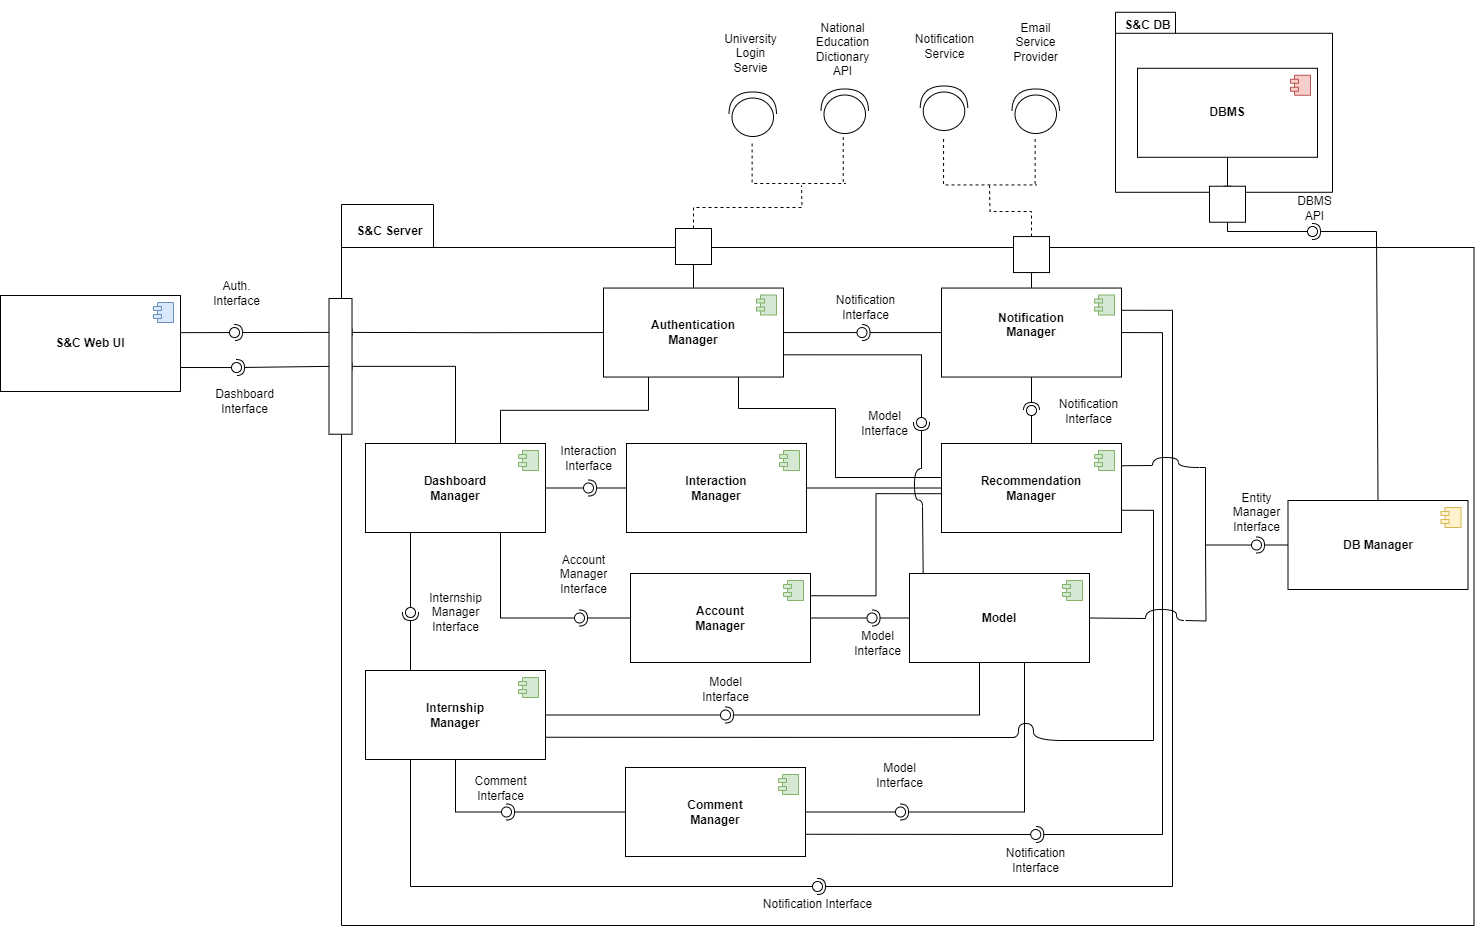
\includegraphics[scale=0.50]{DD_figures/S&C.drawio.png}\\
\caption{Component Diagram of the S\&C-SP subsystem}
\end{sidewaysfigure}
\begin{enumerate}
    \item {C1 Dashboard Manager} :
    \\It's used as an intermediary between the WebUI and the
    other components of the server to provide the web application only the functionality
    strictly necessary for it to work properly.
    \item {C2 Account Manager} :
    \\This component handles the operations needed to manage each User's account, and to view the Users' profiles. It allows Users to login, using the Authentication Manager's interface.
    \item {C3 Authentication Manager} :
    \\This component handles signup, login and logout operations.
    \item {C4 Internship Manager} :
    \\This component handles the operations needed to manage an Internship, to view any information about it and to accept it.
    \item {C5 Comment Manager} :
    \\This component handles the operations needed to view and write comments (complaints and observations.
    \item {C6 Recommendation Manager} :
    \\This component is responsible for the recommendation mechanism for students and internships. It takes the input data from the user interactions with the system and reloads the associated recommendations.
    \item {C7 Interaction Manager} :
    \\This component is responsible for registering feedbacks and interactions of the user with the web application, transforming this information into parameters, and passing it to the recommendation manager for elaboration.
    \item {C8 Notification Manager} :
    \\This component is responsible for the dispatch of notifications.
    \item {C9 Model} :
    \\This component facilitates the interaction with and representation of S\&C-SP data.
\end{enumerate}
\subsection{Deployment View}
We adopted a 3-tier architecture hosted on cloud infrastructure, designed to optimize performance and scalability while reducing costs.

Let's explore more in detail:

\begin{enumerate}
    \item \textbf{Scalability and Flexibility} - the ability to add or remove resources such as virtual machines, performance cores, or memory as needed, in conjunction with the use of load balancing services, allows the servers to adapt to changes in traffic or workload.
    \item \textbf{Security} - Firewalls help to protect the application server against data breaches and other security threats.
    \item \textbf{Cost-efficiency} - the choice of using a cloud provider allows us to only pay for the resources that we are actually using, which can help to lower the overall costs, and in general reduces the waste of resources.
\end{enumerate}

The cloud provider is an ideal choice for hosting large, high-traffic applications. The chosen cloud provider will need to offer all of these features in order to meet our needs.

The web server resides in the De Militarized Zone and is the primary interface for user interaction. The application server executes the core application logic, processing user requests and handling all the operations. Load balancers are implemented to evenly distribute incoming traffic across multiple instances of Web and Application Servers.
\begin{figure}[H]
    \centering
    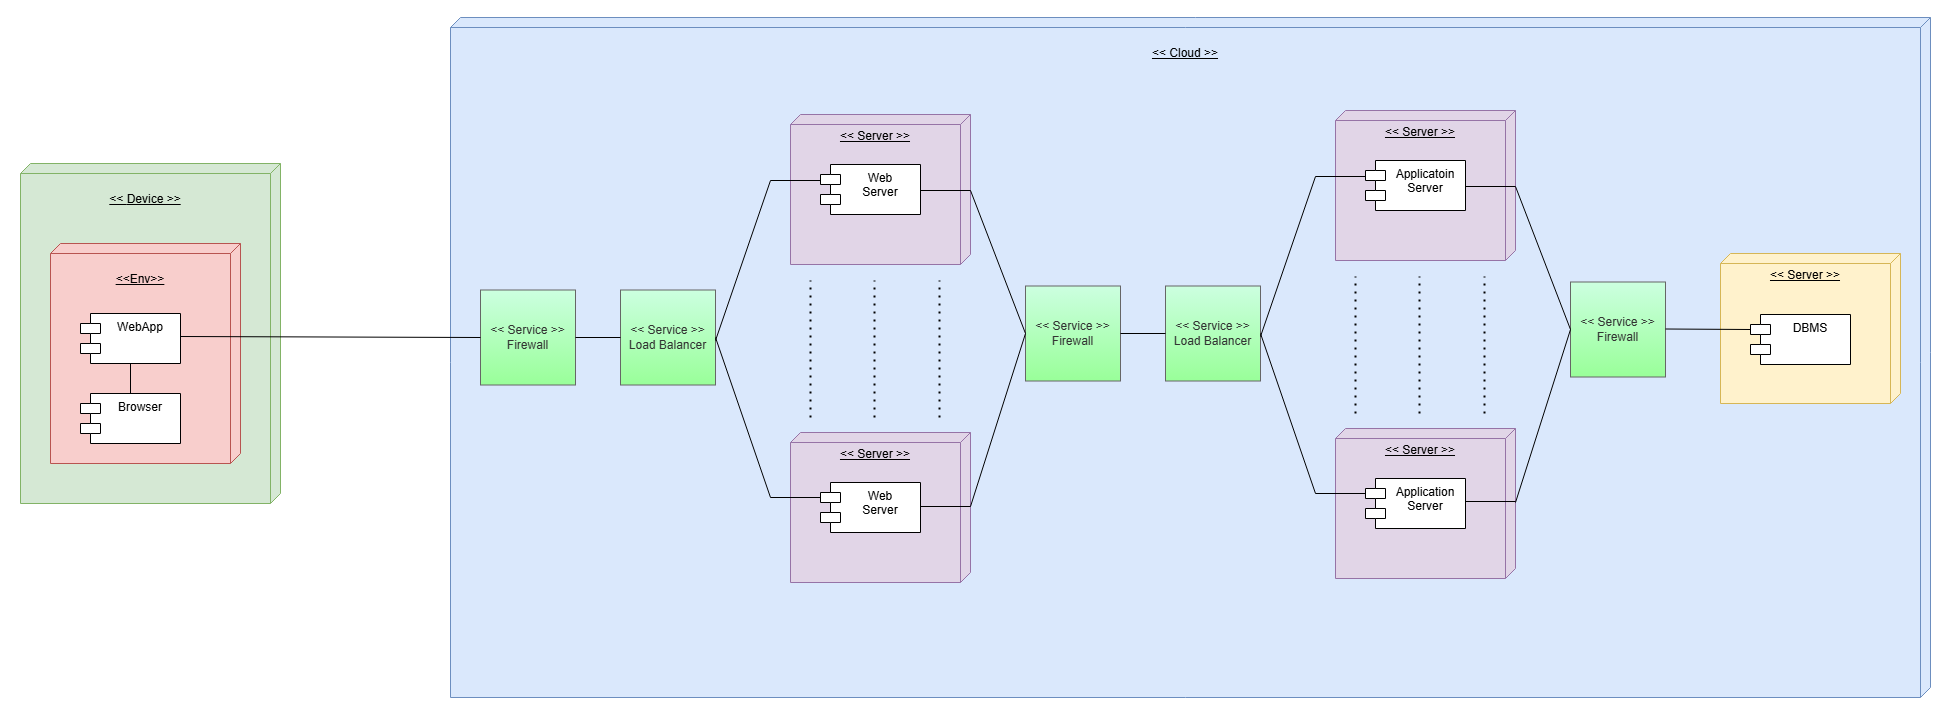
\includegraphics[scale = 0.33]{DD_figures/SingleDiagrams/DeploymentView.png}
    \caption{Component Diagram of the S\&C server subsystem}
    \centering
\end{figure}


\subsection{Runtime View}

\subsubsection*{Student Registers}
The diagram represented below shows the process of a Student creating an account to the S\&C website. First, the Student compiles the sign up form with all the requested information. Immediately after, the University login service, related to the university that the Student inserted in the form, is shown. If the Student logs successfully in its university account then the form information is stored in the DB and a new account is generated. From there, the AuthenticationManager triggers the verification email through the EmailServiceProvider. Eventually, all the companies that advertise an internship that system recognizes valid to recommend are notified of the new student subscription to the platform.
\begin{figure}[H]
\centering
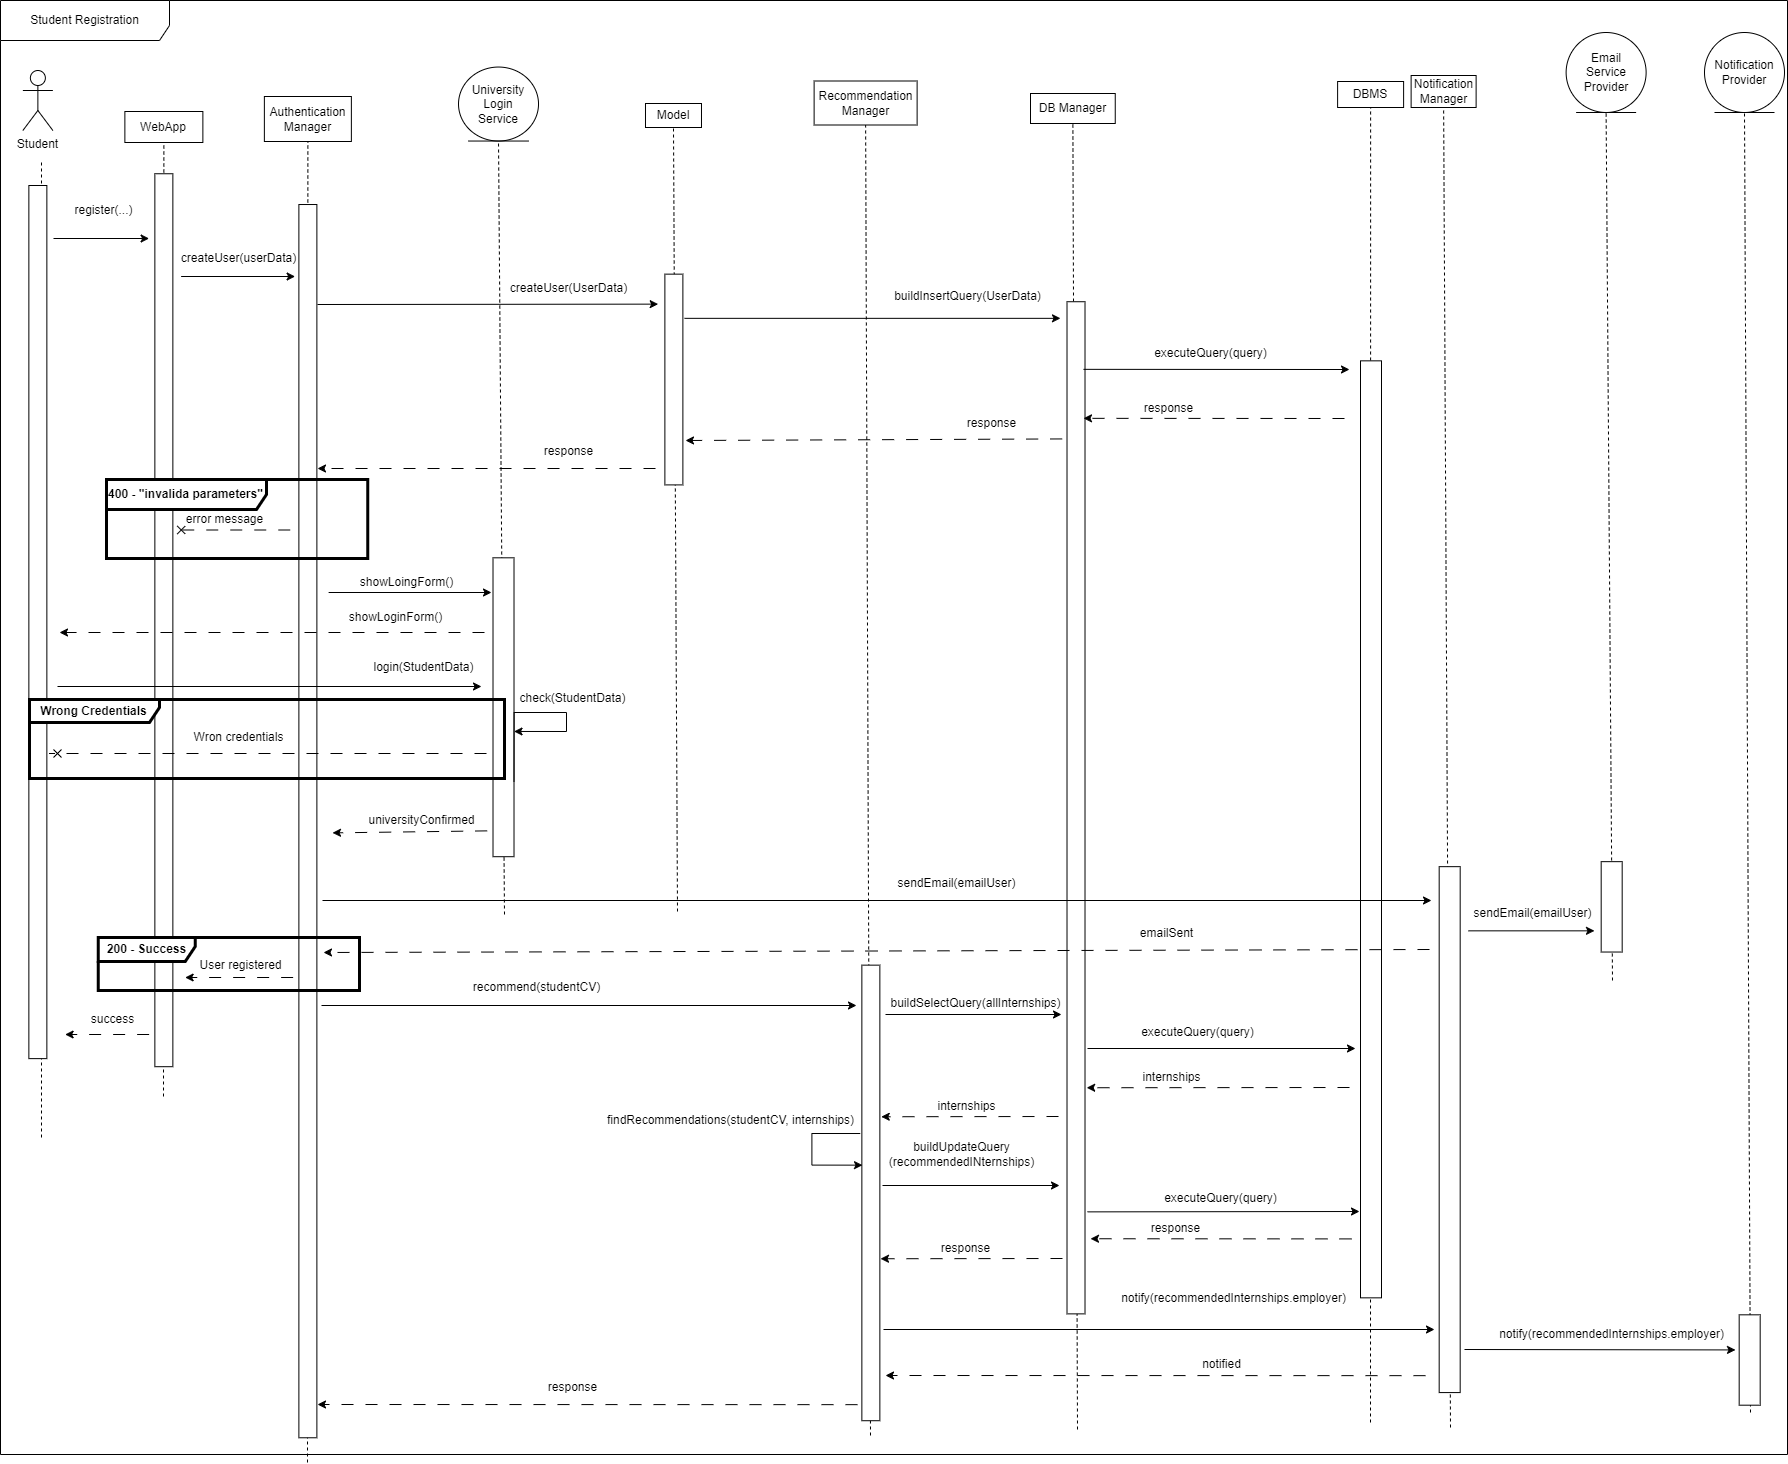
\includegraphics[scale = 0.28]{DD_figures/RuntimeView/StudentRegistrationRV.drawio.png}\\
\caption{Student registers to S\&C}
\end{figure}

\subsubsection*{Company Registers}
The diagram represented down below shows the process of a Company creating an account to the S\&C website. First, the Company compiles the sign up form with all the requested information, then, as the request is submitted through the proper API call, the AuthenticationManager component handles the request, and, if the parameters of the request were valid, the AuthenticationManager
triggers the verification email through the EmailServiceProvider.
\begin{figure}[H]
\centering
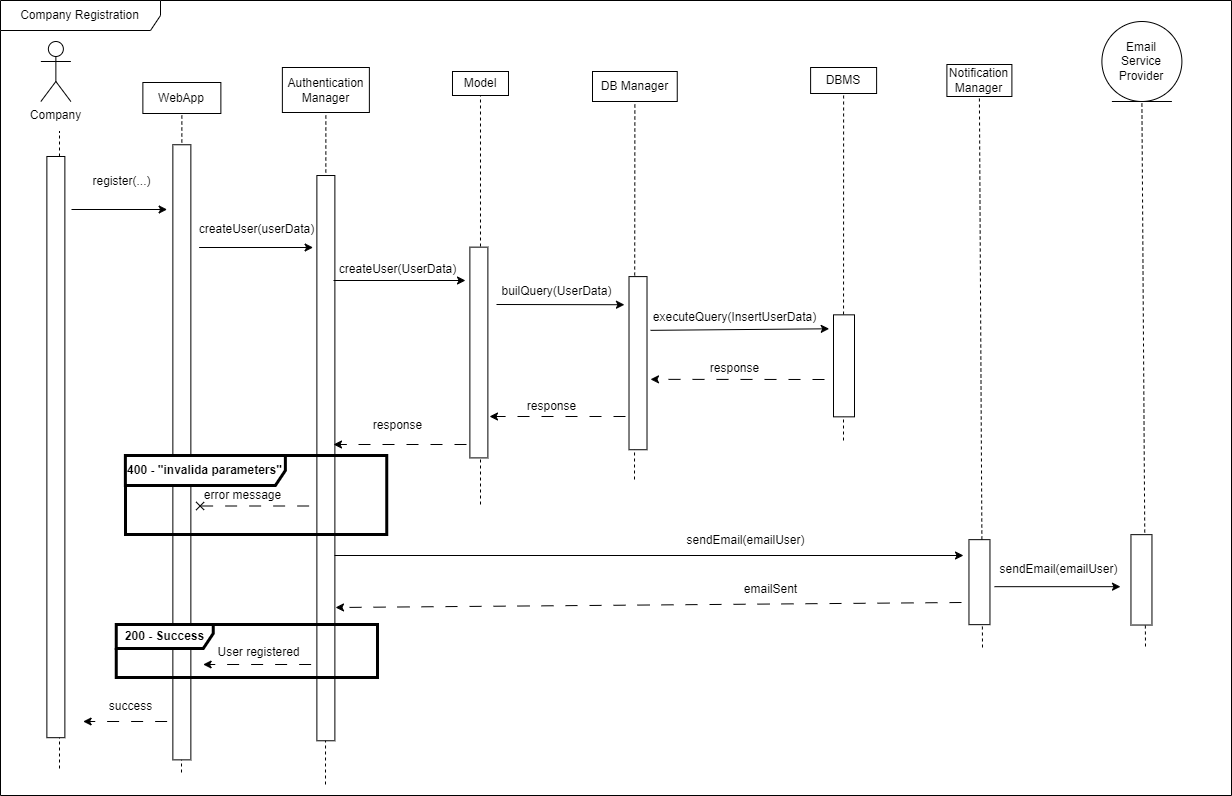
\includegraphics[scale = 0.42]{DD_figures/RuntimeView/CompanyRegistersRV.drawio.png}\\
\caption{Company registers to S\&C}
\end{figure}

\subsubsection*{University Registers}
The diagram represented down below shows the process of a University creating an account to the S\&C website. First, the University compiles the sign up form with all the requested information. From there, the University information is checked using the National Education Dictionary. If the information results correct, then the information is stored in the DB and a new University account is generated. At last, the AuthenticationManager
triggers the verification email through the EmailServiceProvider.
\begin{figure}[H]
\centering
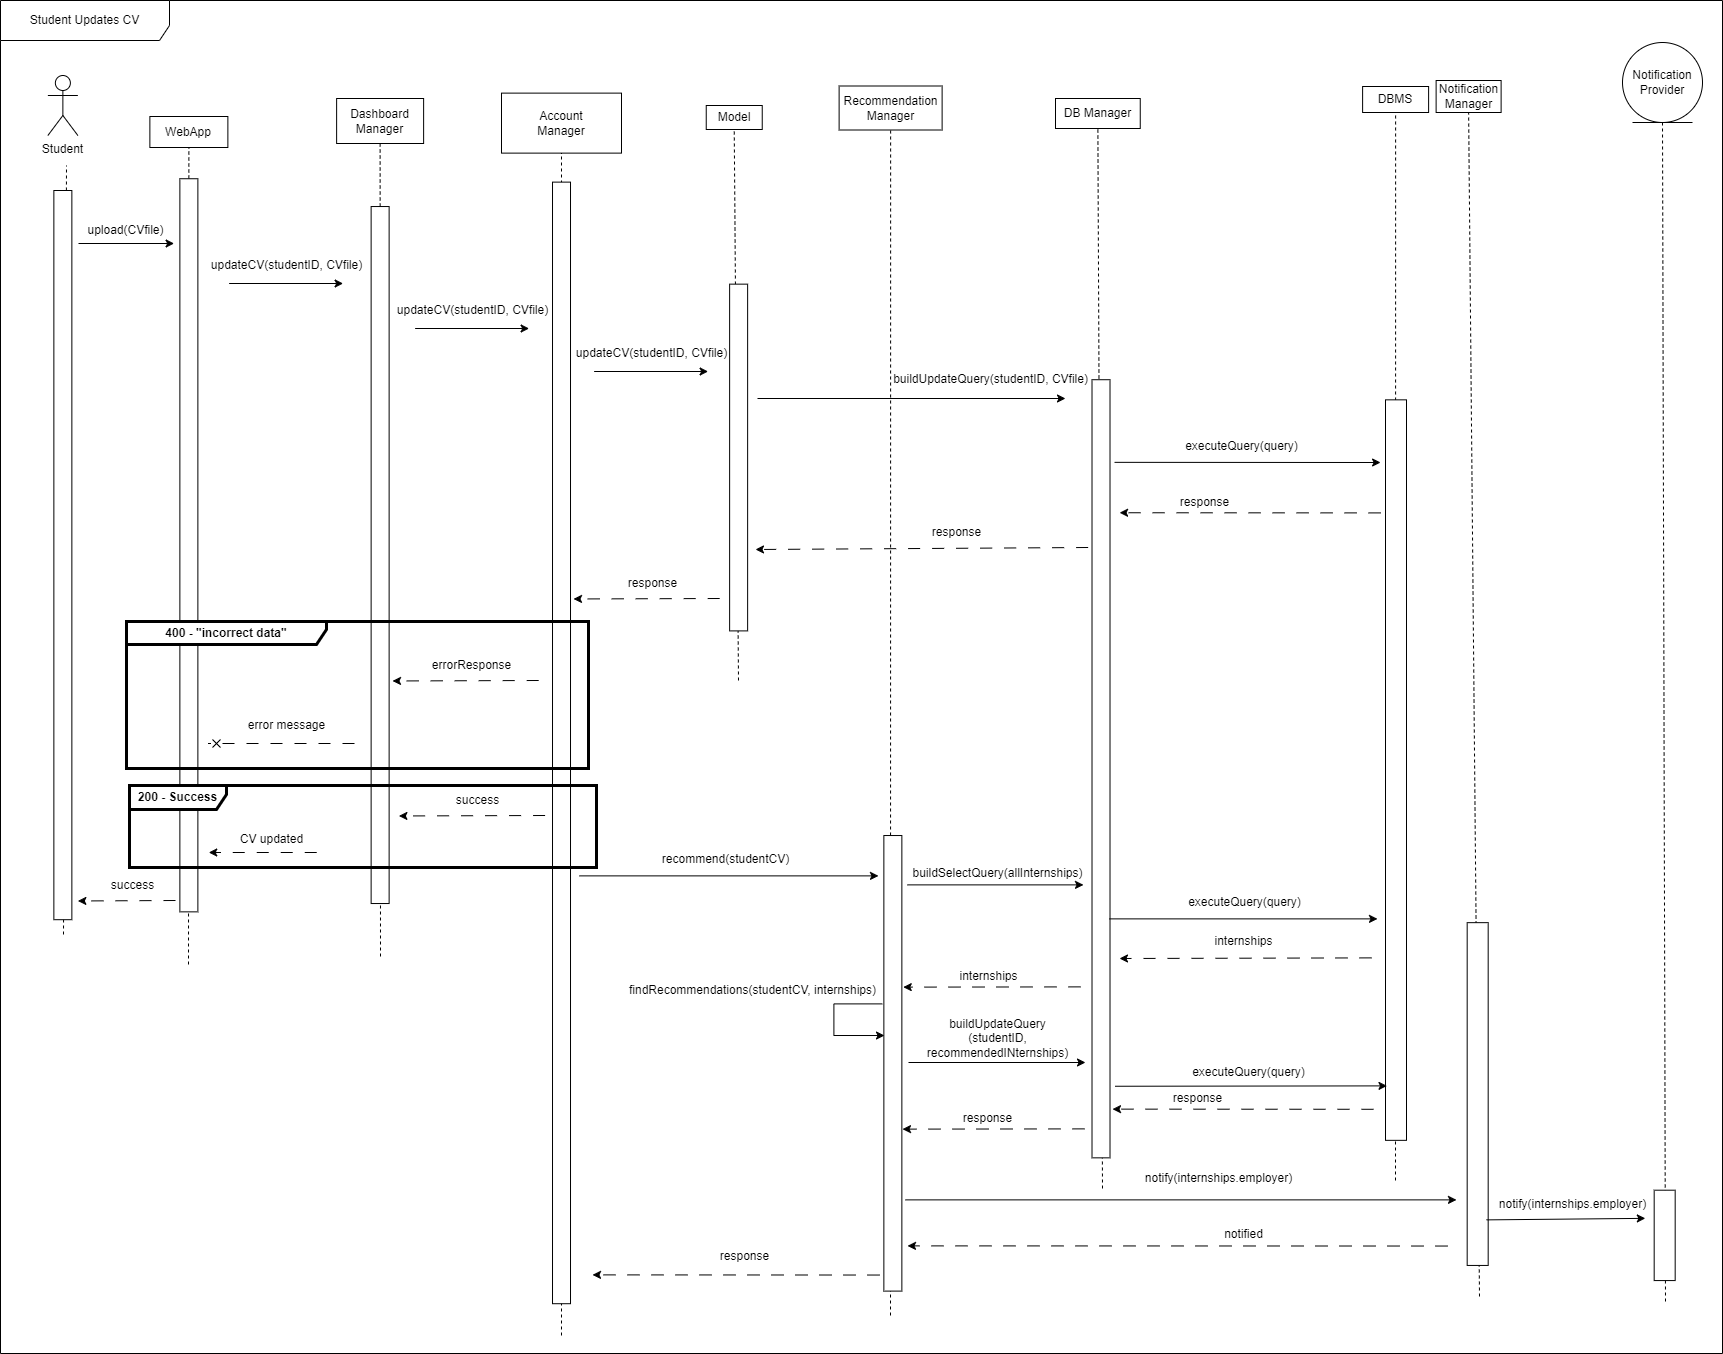
\includegraphics[scale = 0.30]{DD_figures/RuntimeView/StudentUpdatesCV_RV.drawio.png}\\
\caption{university registers to S\&C}
\end{figure}

\subsubsection*{Student Updates CV}
The student initiates the process by uploading their CV, which is handled by the WebApp and subsequently passed to the Dashboard Manager, Account Manager, and Model components for validation and processing. If the data is valid, the CV is updated in the database using a query managed by the DB Manager and DBMS. Upon successful update, the Recommendation Manager generates internship recommendations based on the updated CV, retrieving relevant internships and notifying associated employers. In case of an error (e.g., incorrect data), the system responds with an appropriate error message. Notifications are sent to employers via the Notification Provider, ensuring the flow of updates and recommendations.
\begin{figure}[H]
\centering
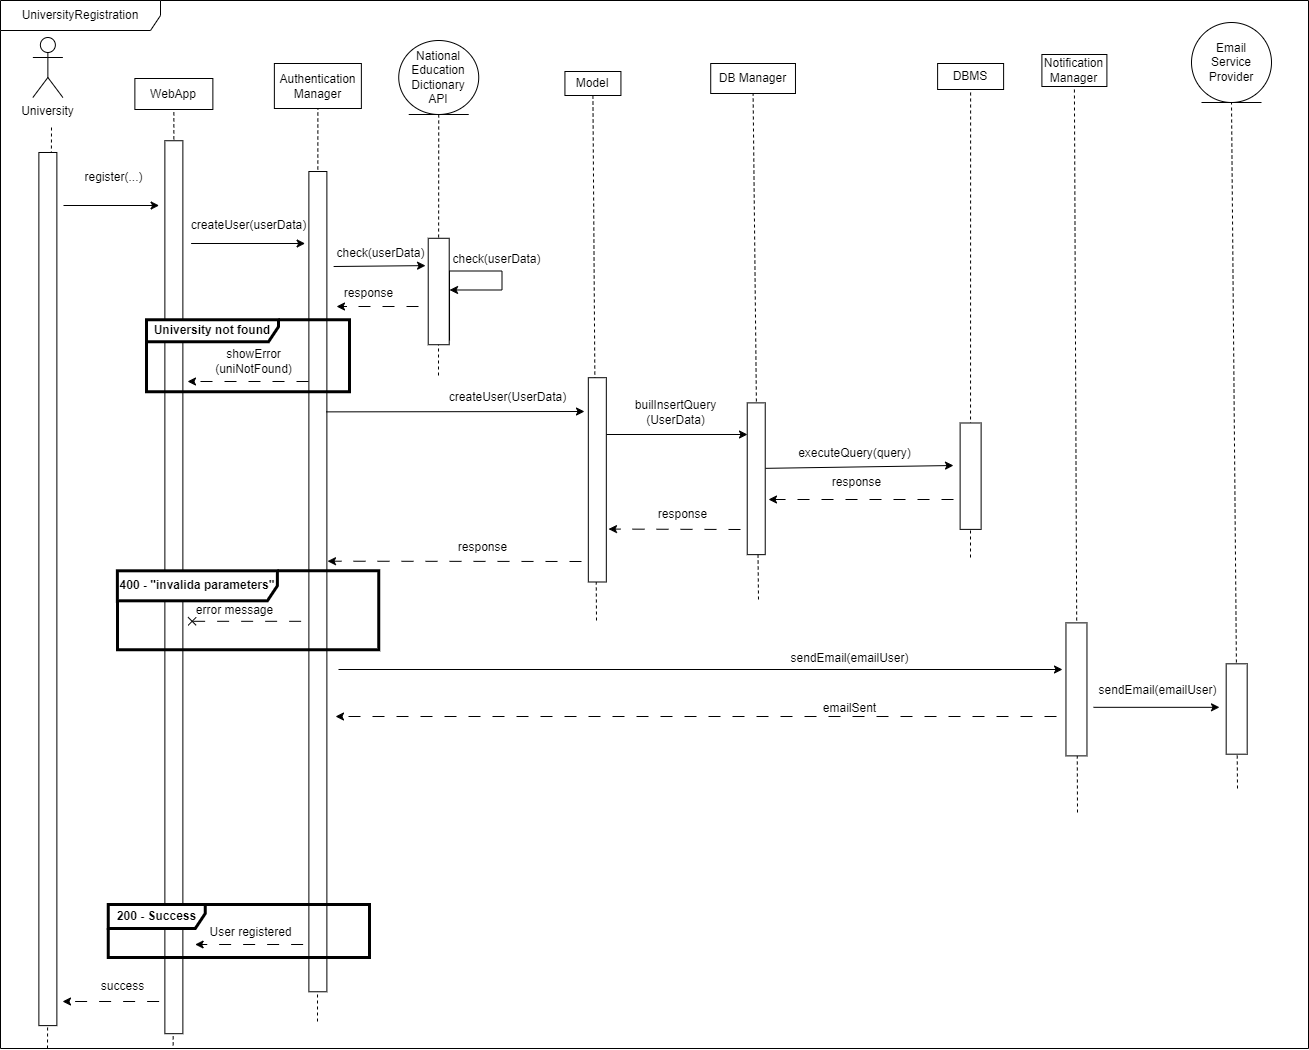
\includegraphics[scale = 0.35]{DD_figures/RuntimeView/UniversityRegistrationRV.drawio.png}\\
\caption{Student Updates CV}
\end{figure}

\subsubsection*{Student changes university}

\begin{figure}[H]
\centering
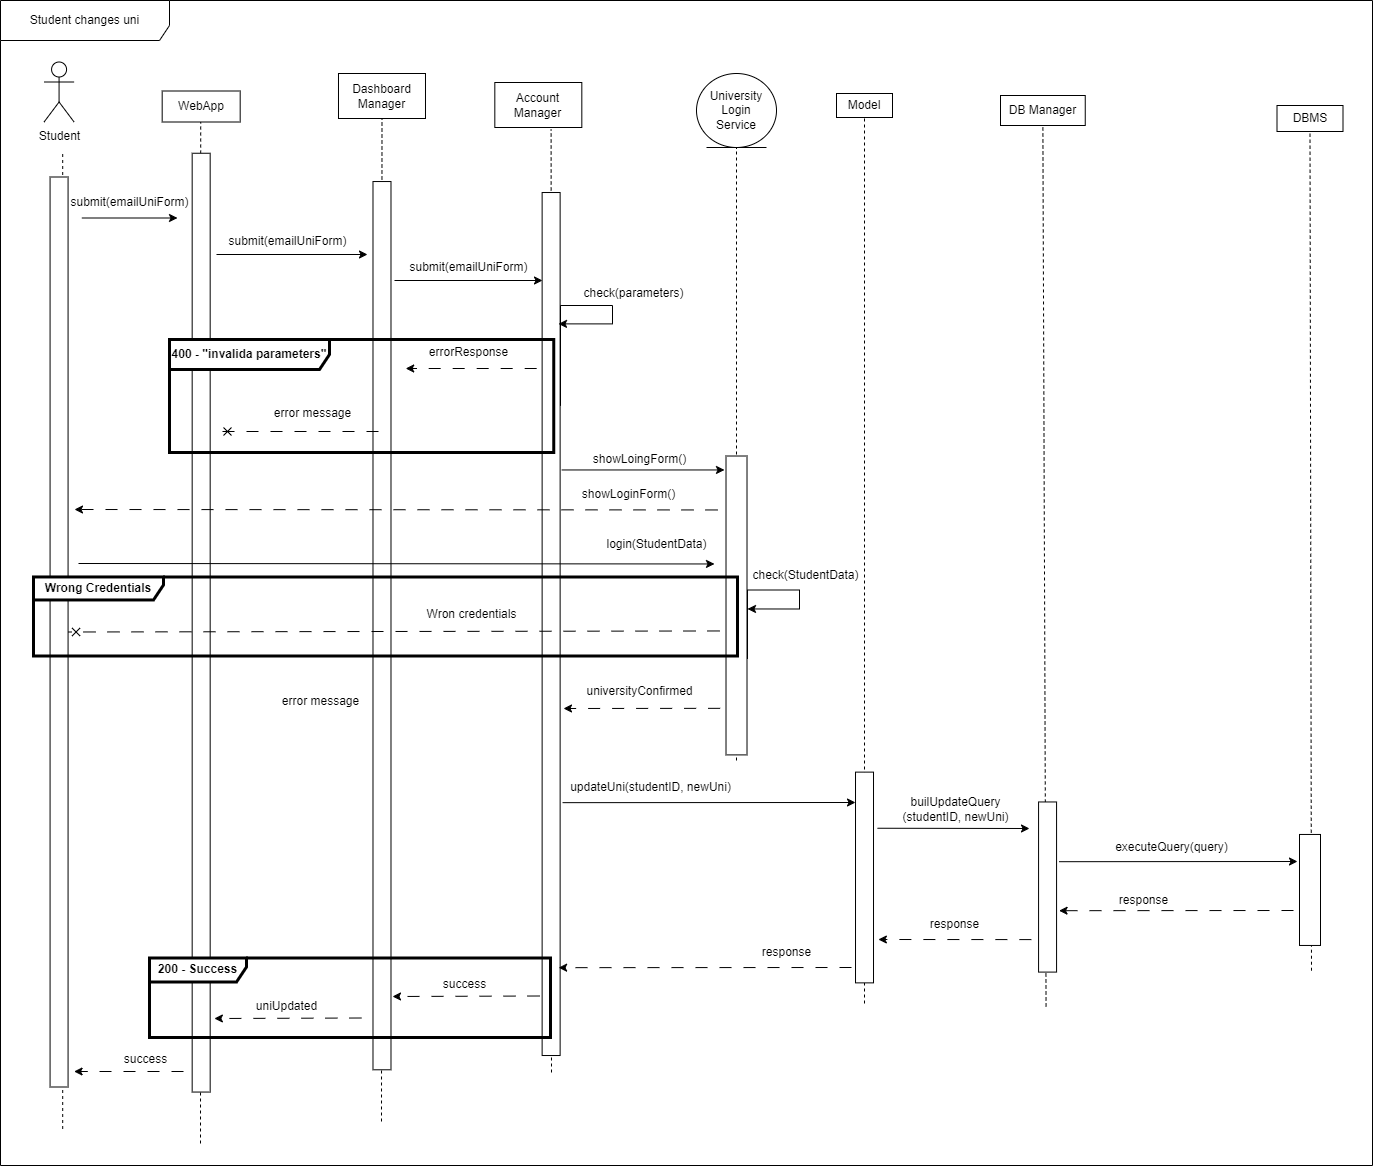
\includegraphics[scale = 0.35]{DD_figures/RuntimeView/StudentChangesUniversityRV.drawio.png}\\
\caption{Student changes university}
\end{figure}

\subsubsection*{Company sends interview form}

\begin{figure}[H]
\centering
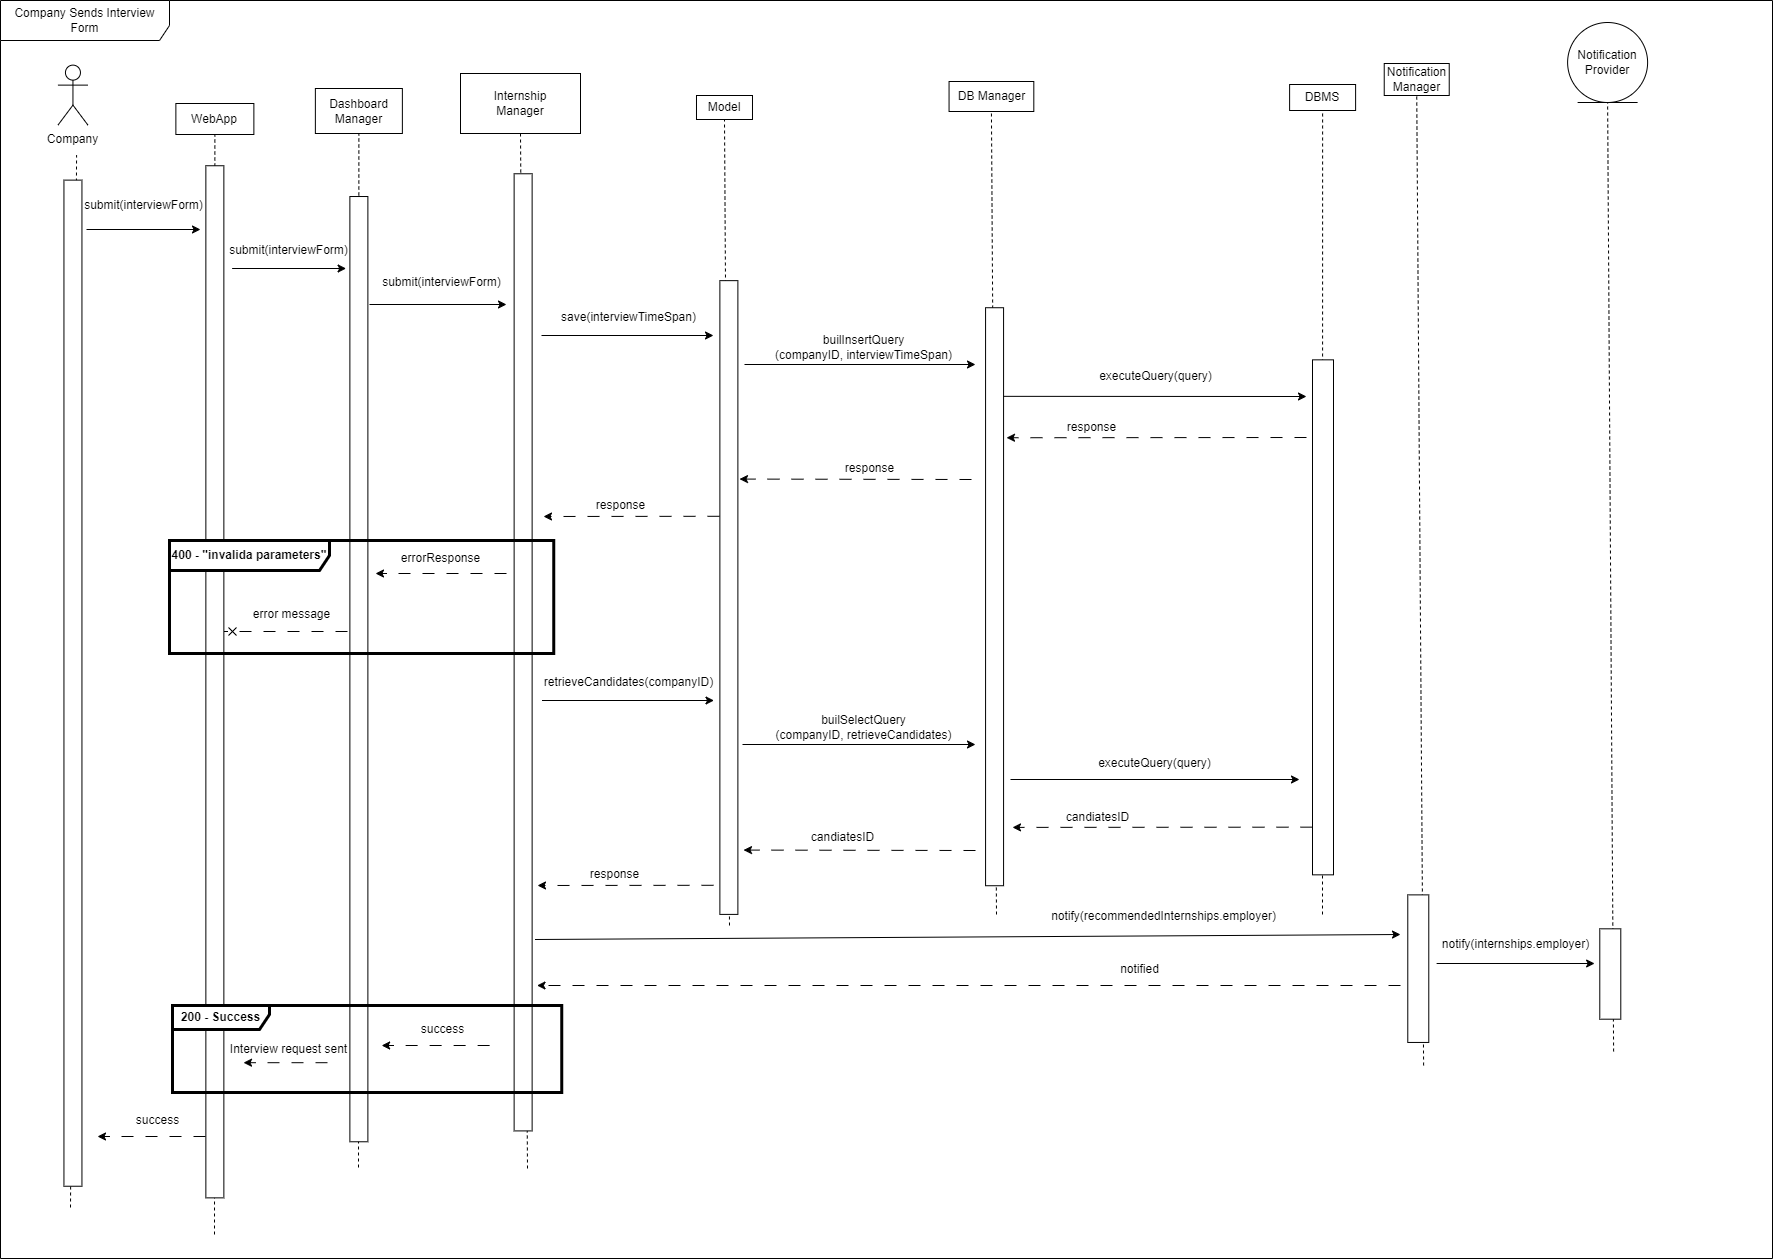
\includegraphics[scale = 0.30]{DD_figures/RuntimeView/CompanySendsInterviewFormRV.drawio.png}\\
\caption{Company sends interview form}
\end{figure}

\subsubsection*{Student selects interview date}

\begin{figure}[H]
\centering
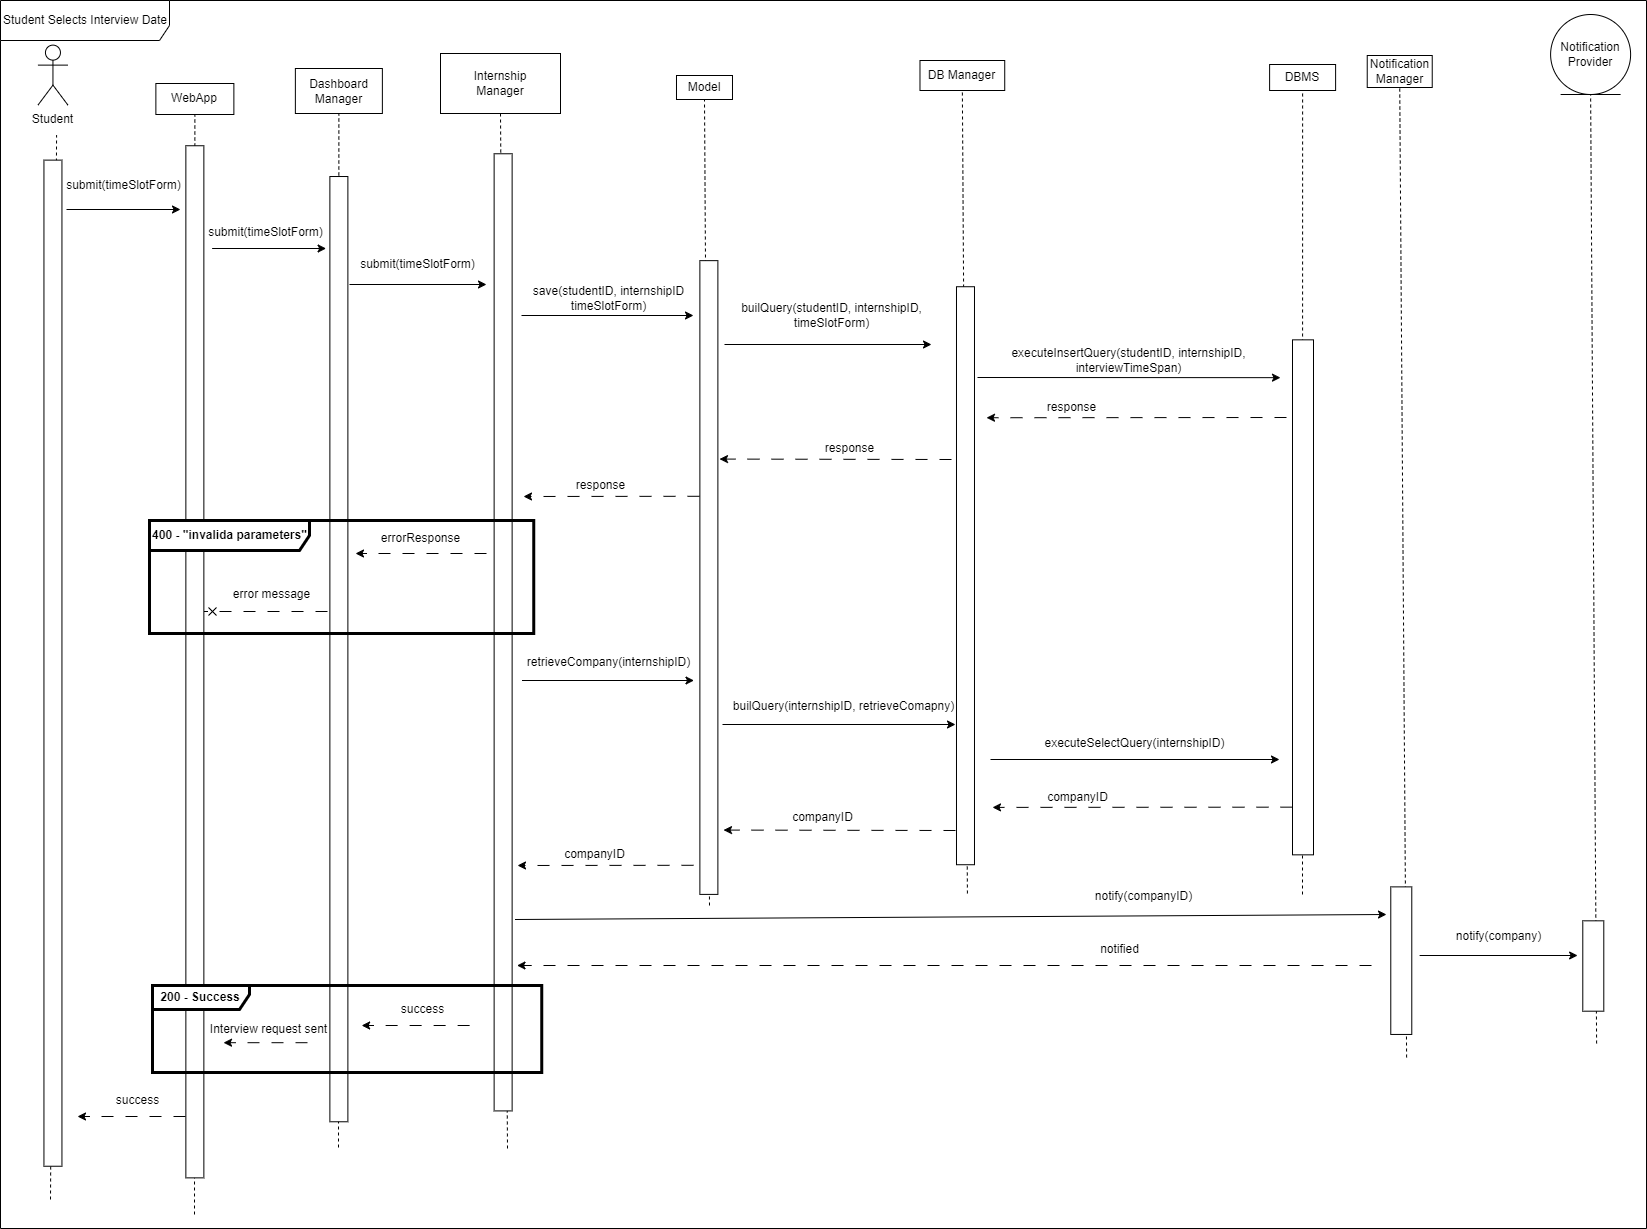
\includegraphics[scale = 0.30]{DD_figures/RuntimeView/StudentSelectsInterviewDateRV.drawio.png}\\
\caption{Student selects interview date}
\end{figure}

\subsubsection*{Company selects candidate}

\begin{figure}[H]
\centering
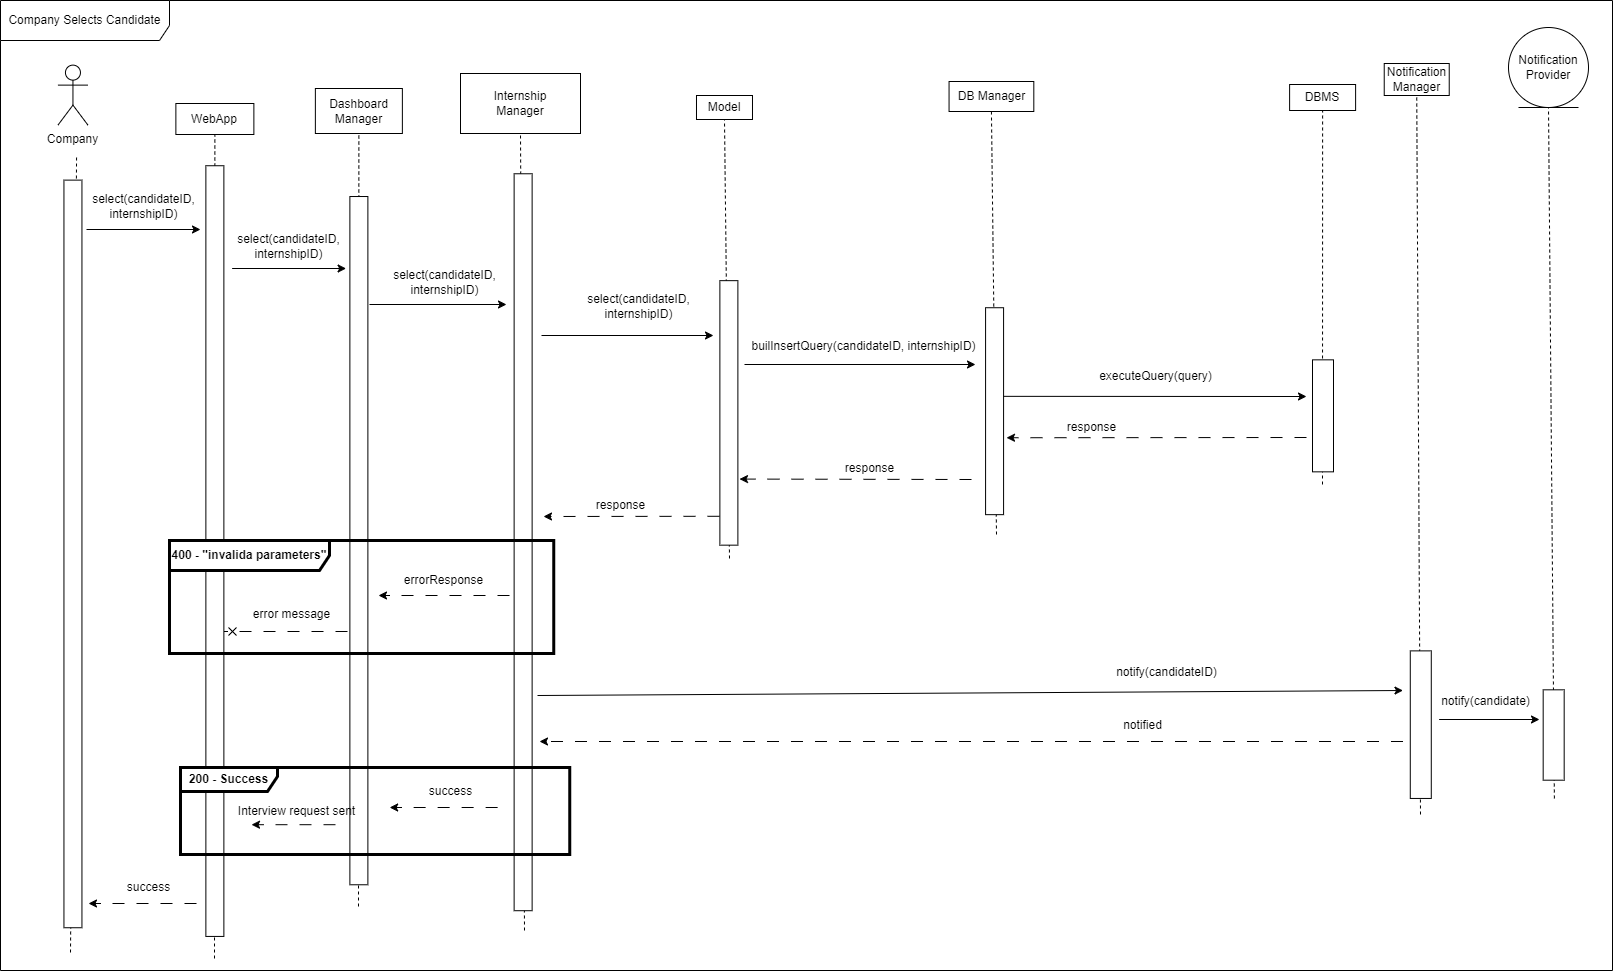
\includegraphics[scale = 0.30]{DD_figures/RuntimeView/CompanySelectsCandidateRV.drawio.png}\\
\caption{Company selects candidate}
\end{figure}


    
    \subsubsection*{ User Login}
    This diagram illustrates the login process within the system, regardless of the user type. We assumed that the user identifies their own type through interfaces and navigates the event flow using specific tabs and buttons to ultimately reach the login page. 
    
    The system verifies the user's credentials by querying with the database through the Authentication Manager. If the provided credentials (email and password) are incorrect, the user encounters an error message with error handling mechanisms  as shown in the diagram. However, if the credentials are valid, the authorized managers retrieve the user's Id from the database and redirect to the user's home page by using that.
    
    In addition, the diagram includes a loop representation to prevent that the potential database errors do not affect the system's overall functionality.
    \begin{figure}[H]
    \centering
    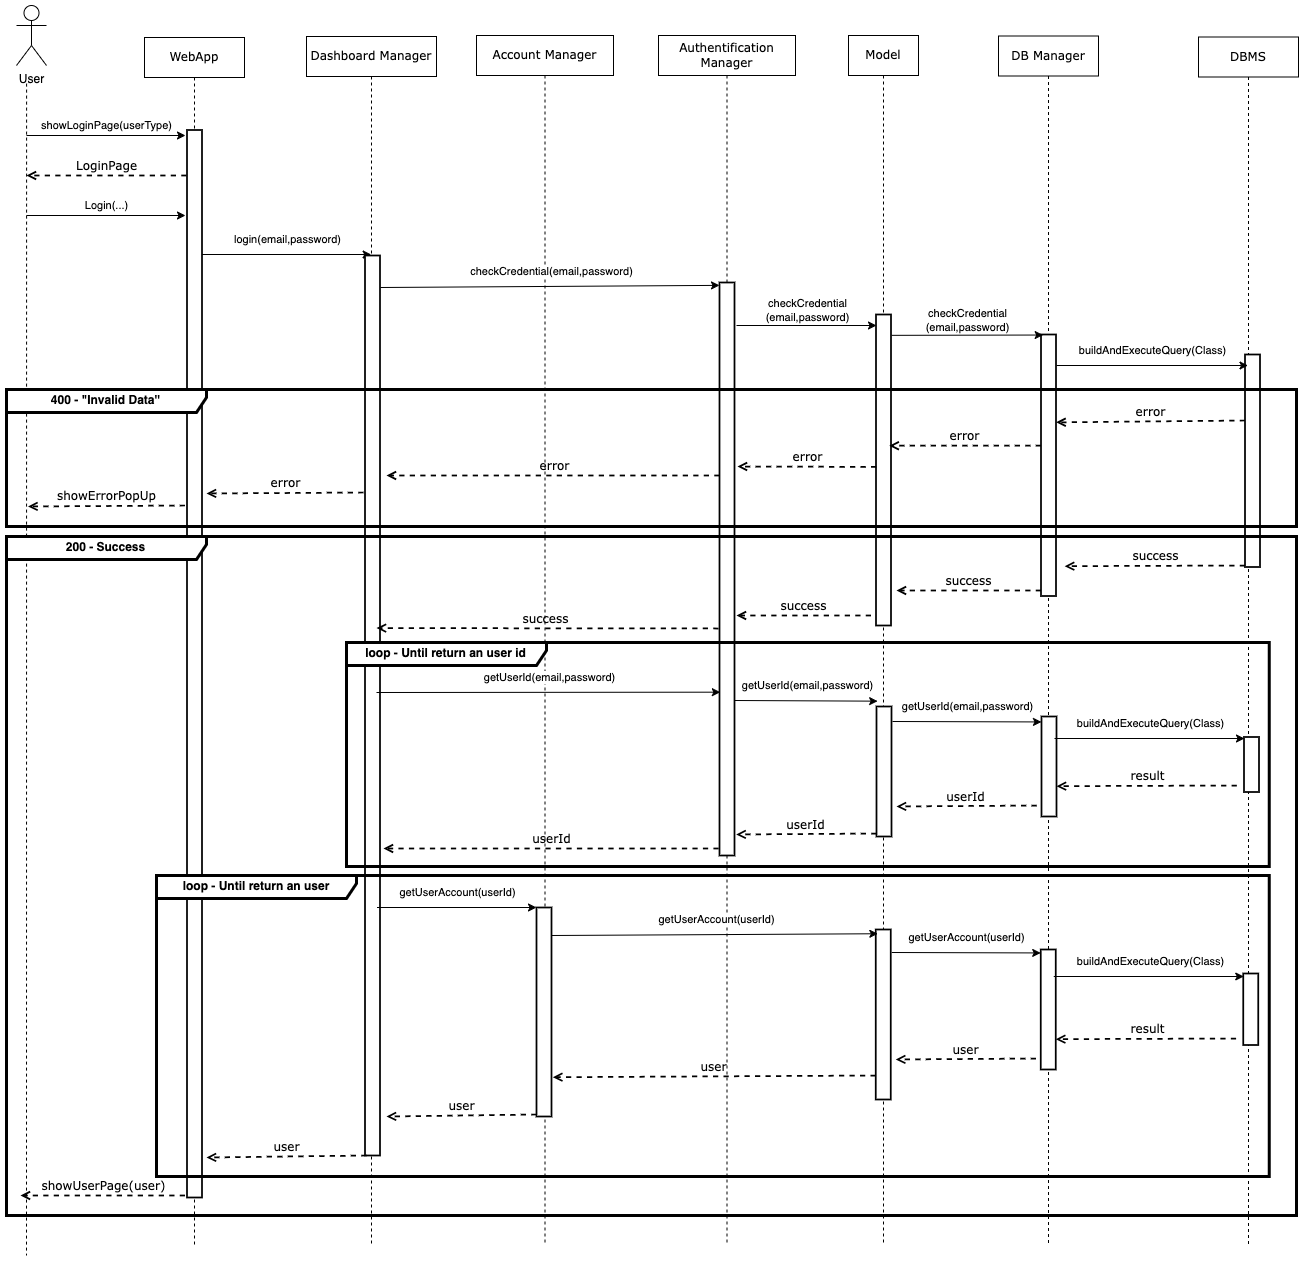
\includegraphics[scale = 0.35]{DD_figures/RuntimeView/UserLogin.drawio.png}
    \caption{User Login}
\end{figure}

\begin{figure}[H]
    \centering
    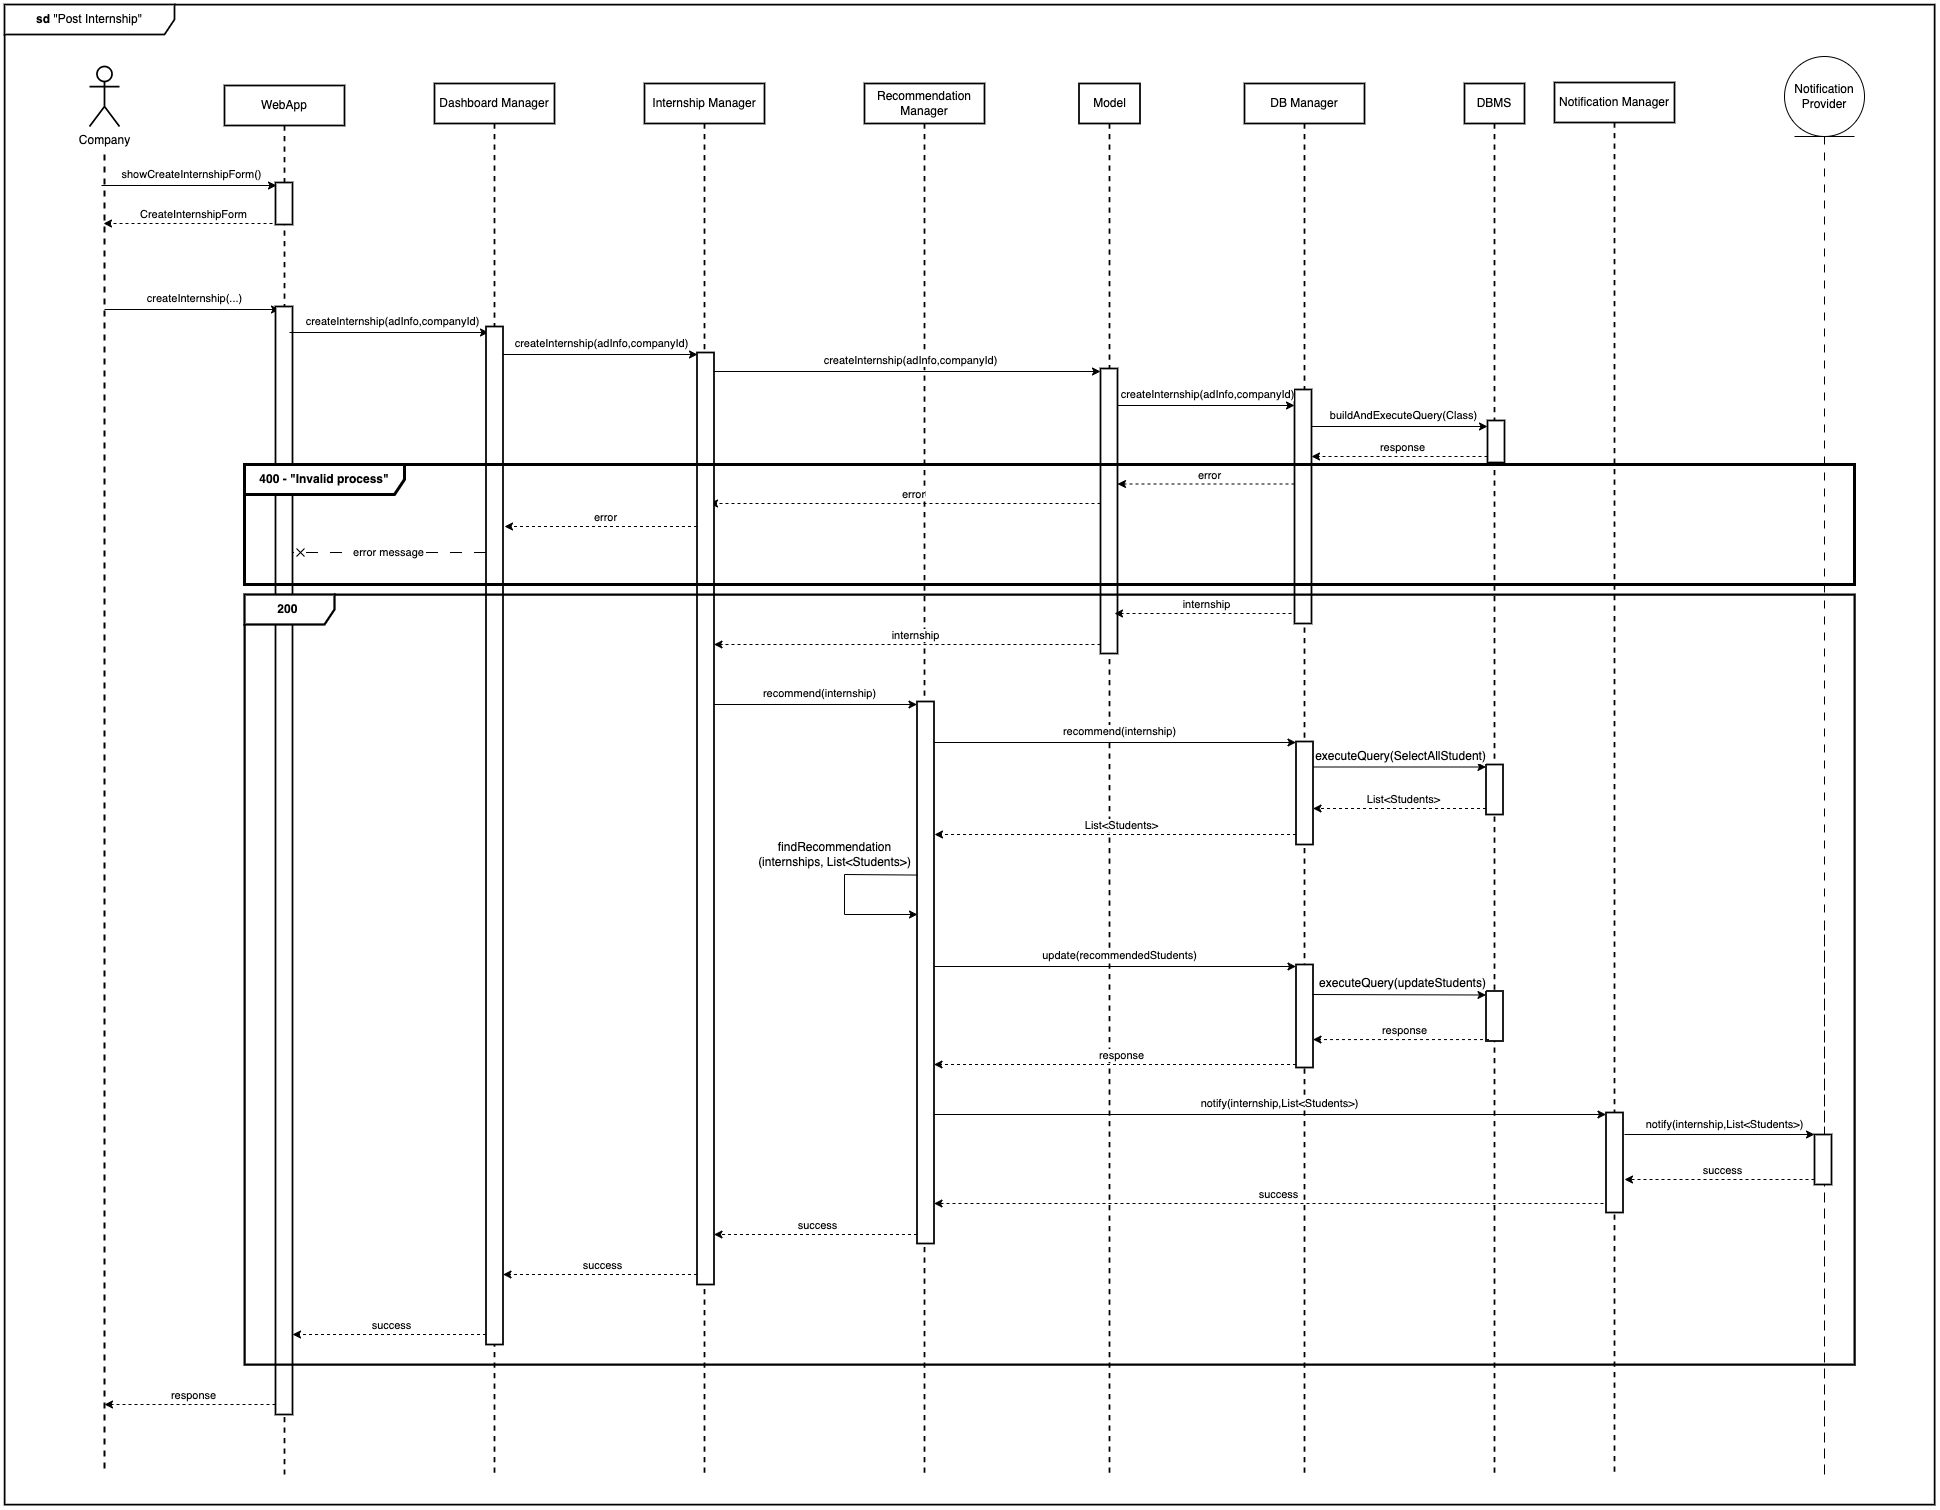
\includegraphics[scale = 0.25]{DD_figures/SingleDiagrams/postInternship.drawio.png}
    \caption{Company Create Internship}
    \centering
\end{figure}
\newpage

\subsubsection*{User Views Relevant Internships}
The diagram below shows the process of a user visualizing the list of internships he's interested in. \\
In the case of a University, it retrieves all the interships the students from that university were selected for
\begin{figure}[H]
\centering
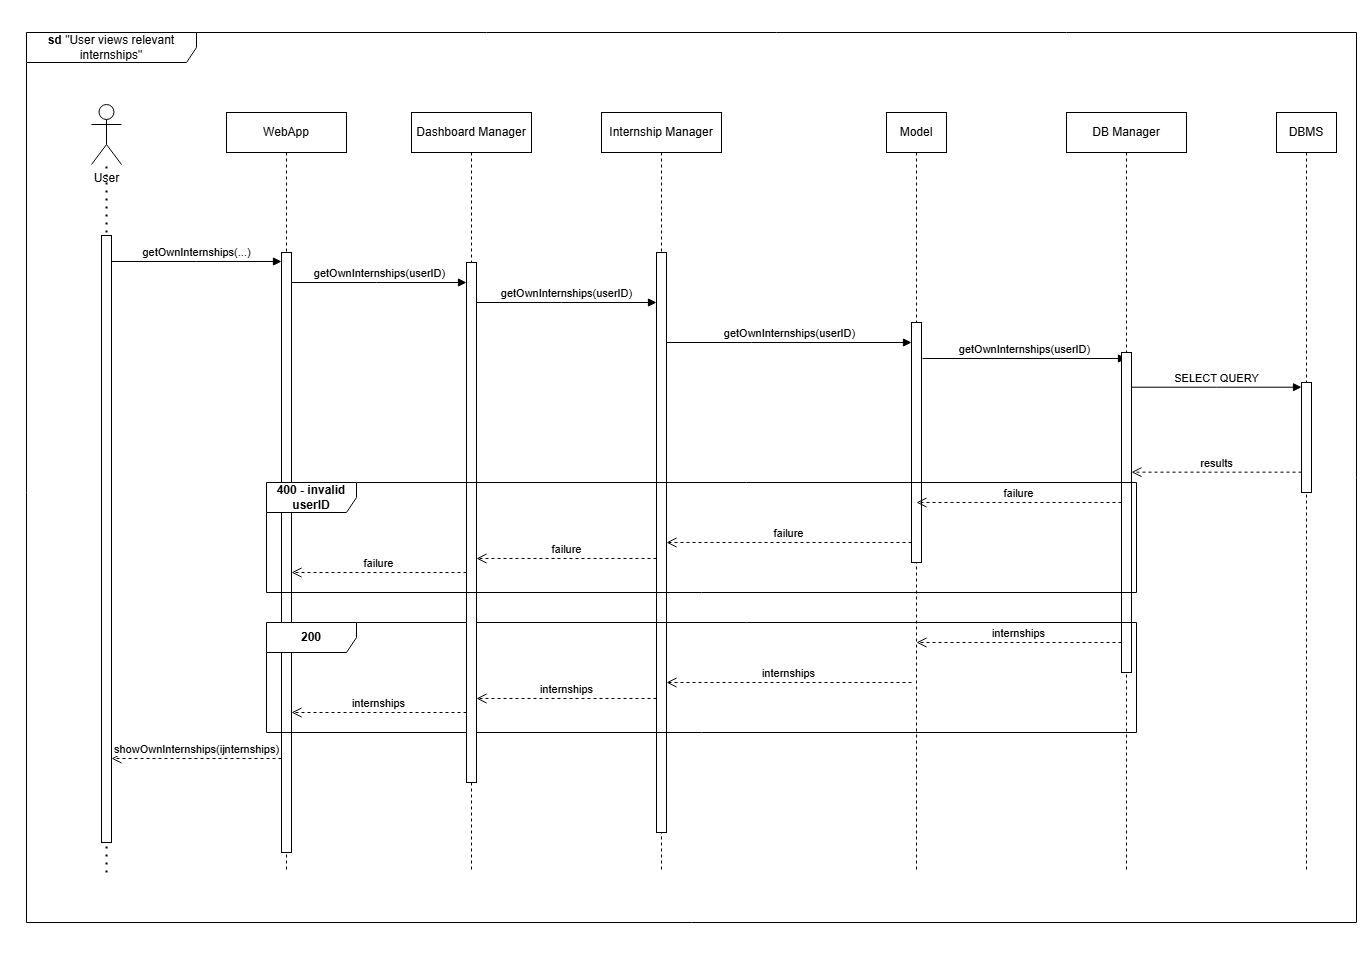
\includegraphics[scale = 0.4]{DD_figures/RuntimeView/UserViewsRelevantInternshipsRV.png}\\
\caption{User Views Relevant Internships}
\end{figure}
\newpage

\subsubsection*{User Accepts Recommendation}
The diagram below shows the process of a User (either student or university) accepting a recommendation proposed by the platform algorithm. Both studentID and internshipID are needed for the operation.
\begin{figure}[H]
\centering
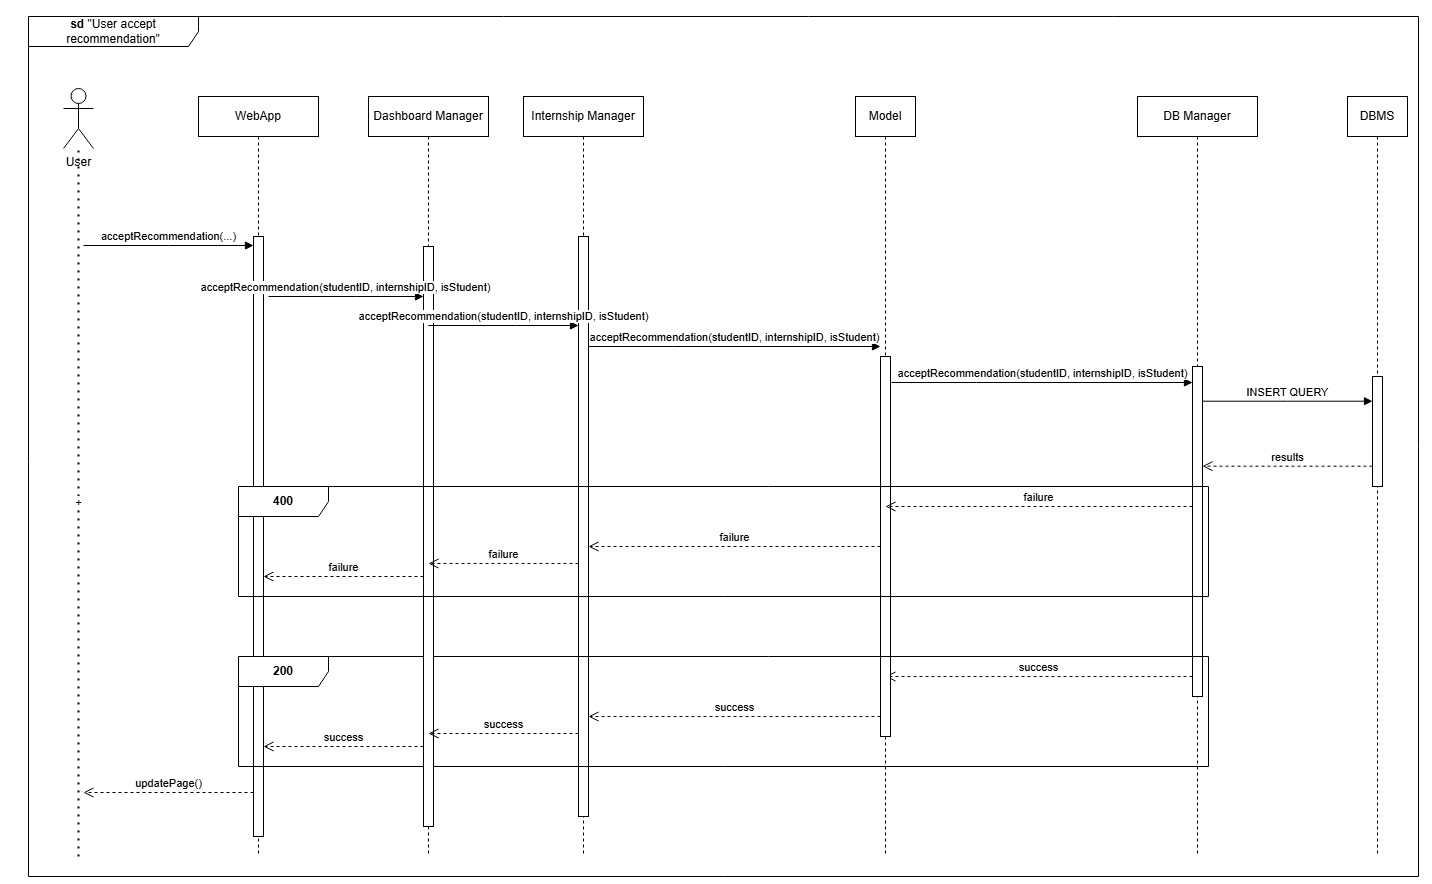
\includegraphics[scale = 0.4]{DD_figures/RuntimeView/UserAcceptsRecommendationRV.png}\\
\caption{User Accepts Recommendation}
\end{figure}
\newpage

\subsubsection*{User Views Comments}
The diagram below shows the process of a User visualizing comments of an internship. If the internshipID is not valid, the process is interrupted.
\begin{figure}[H]
\centering
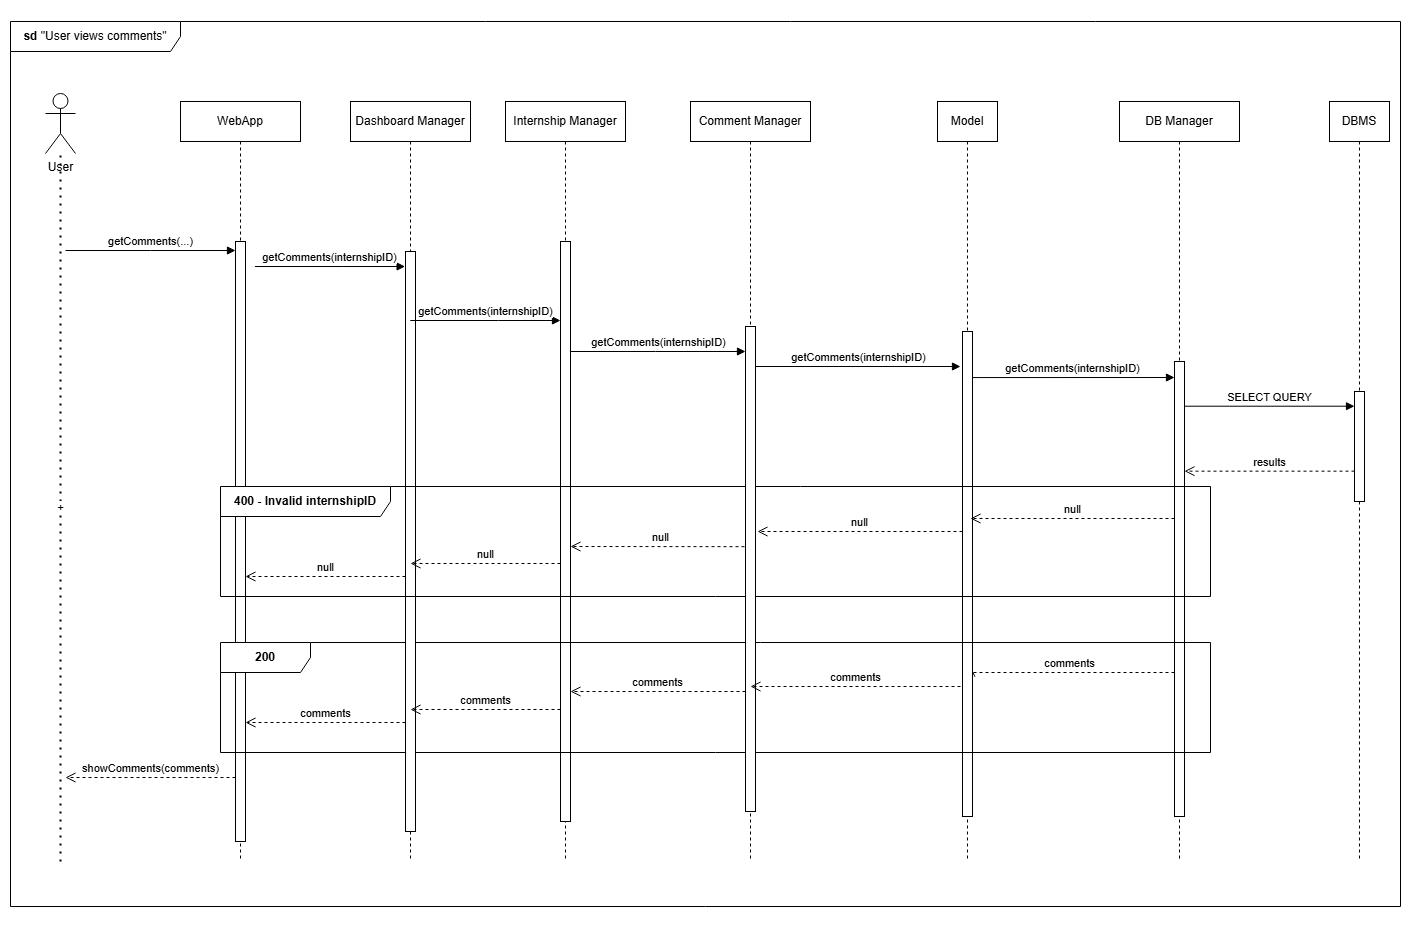
\includegraphics[scale = 0.4]{DD_figures/RuntimeView/UserViewsCommentsRV.png}\\
\caption{User Views Comments}
\end{figure}
\newpage

\subsubsection*{User Writes Observation}
The diagram below shows the process of a User (either student or company) writing an observation about an on-going internship. In this case no notifications are sent, which component will be important for the complaint part.
\begin{figure}[H]
\centering
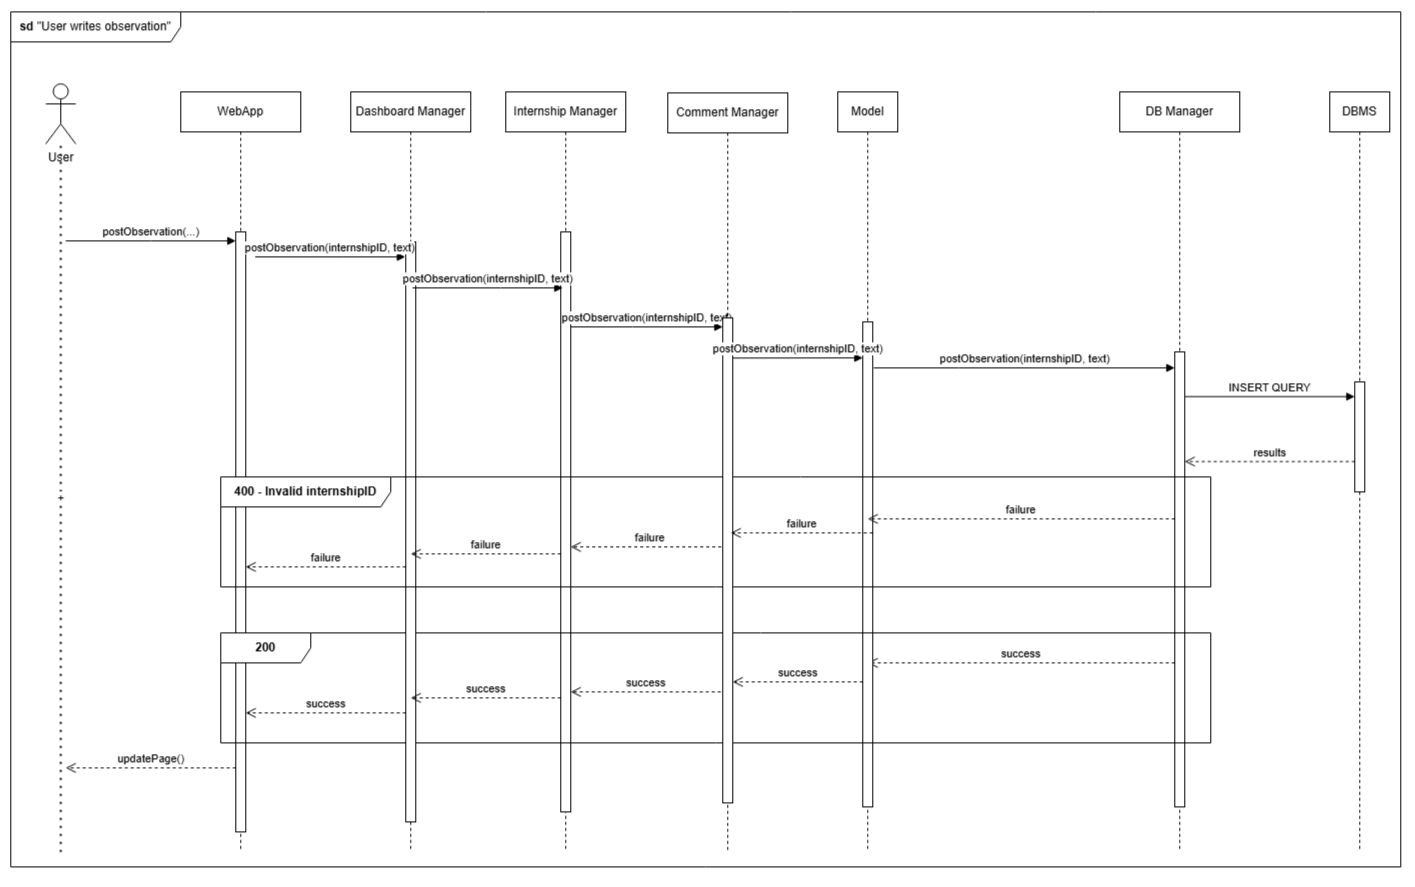
\includegraphics[scale = 0.4]{DD_figures/RuntimeView/UserWritesObservationRV.png}\\
\caption{User Writes Observation}
\end{figure}
\newpage

\subsubsection*{User Writes Complaint}
The diagram below shows the process of a User (either student or company) writing a complaint about an on-going internship. After the complaint has been posted successfully, the system will send a notification to the university of the student that is doing the internship, through the notification provider.
\begin{figure}[H]
\centering
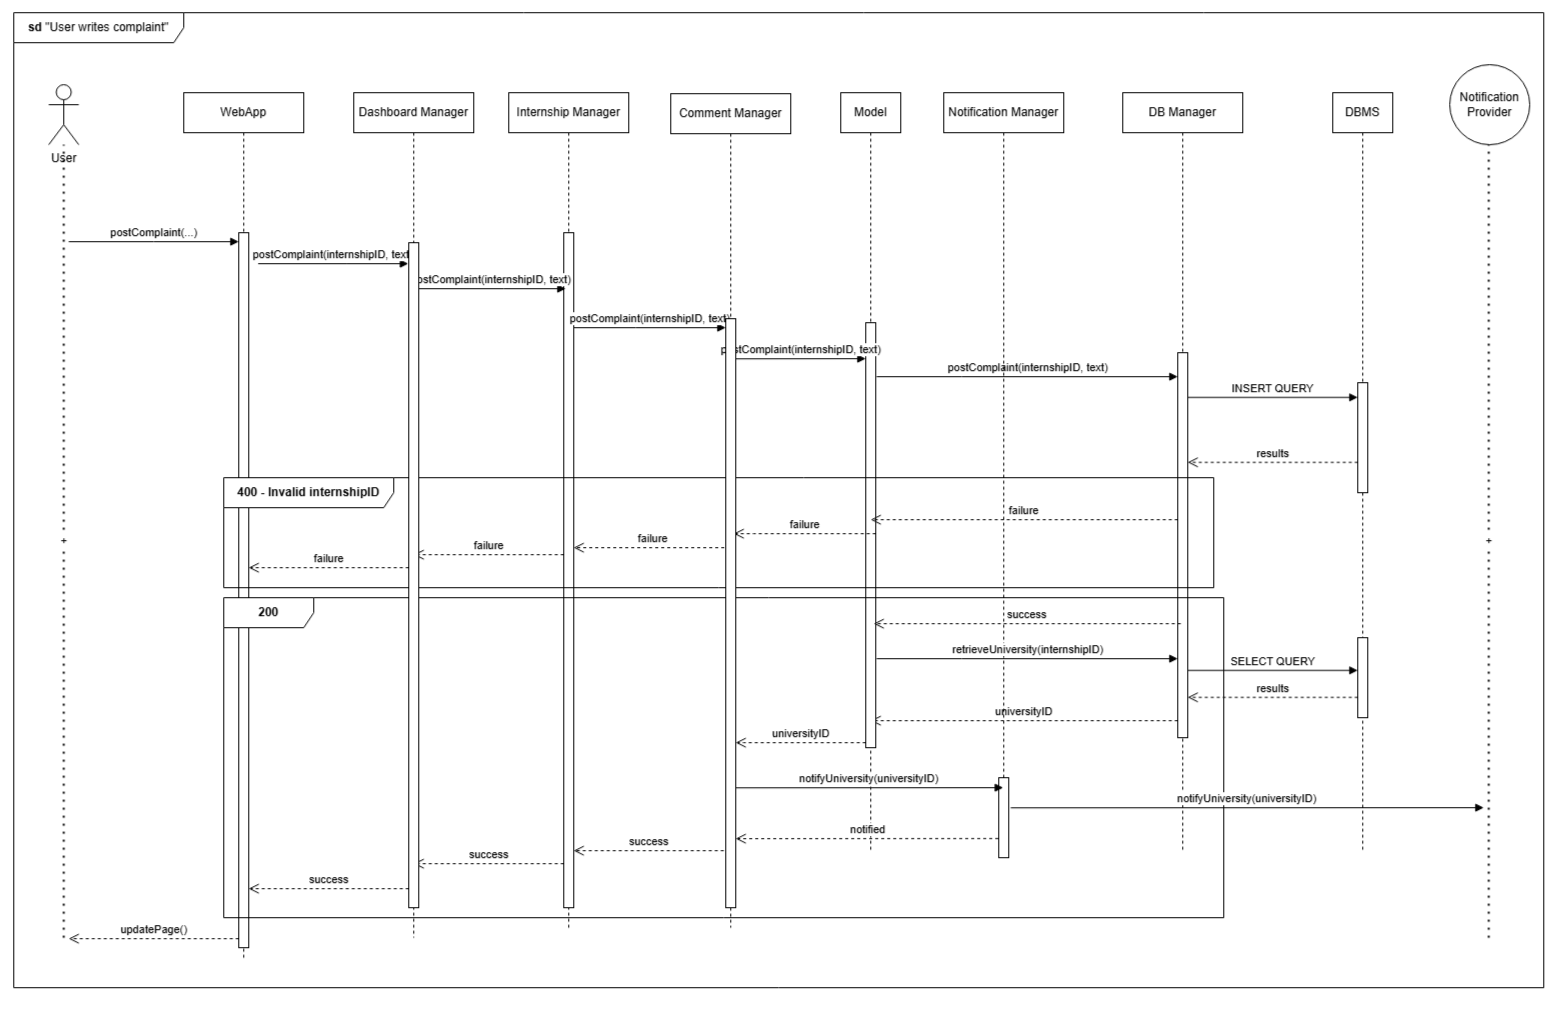
\includegraphics[scale = 0.4]{DD_figures/RuntimeView/UserWritesComplaintRV.png}\\
\caption{User Writes Complaint}
\end{figure}
\newpage

\subsubsection*{University Interrupts Internship}
The diagram below shows the process of a University interrupting an on-going internship. If the internshipID is not valid, the process interrupts. The platform will send notifications to the company and the student relative to that internship.
\begin{figure}[H]
\centering
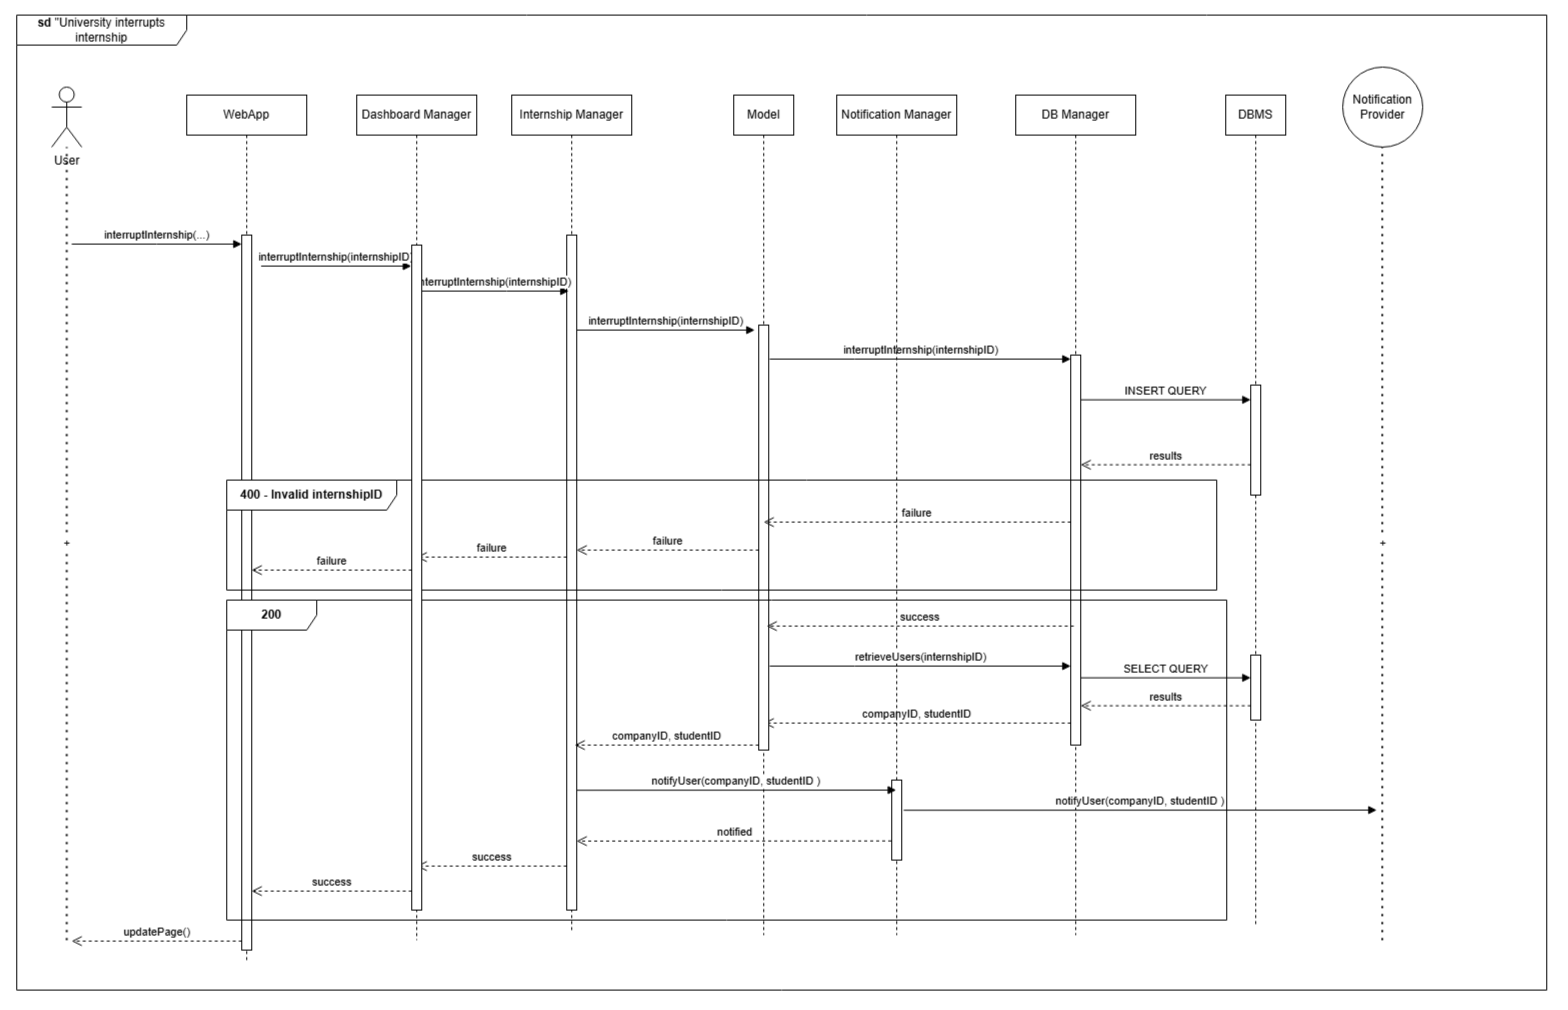
\includegraphics[scale = 0.4]{DD_figures/RuntimeView/UniversityInterruptsInternshipRV.png}\\
\caption{University Interrupts Internship}
\end{figure}
\newpage

\subsubsection*{User Views Template}
The diagram below shows the process of a User (either student or company) visualizing the suggested template by the platform.
\begin{figure}[H]
\centering
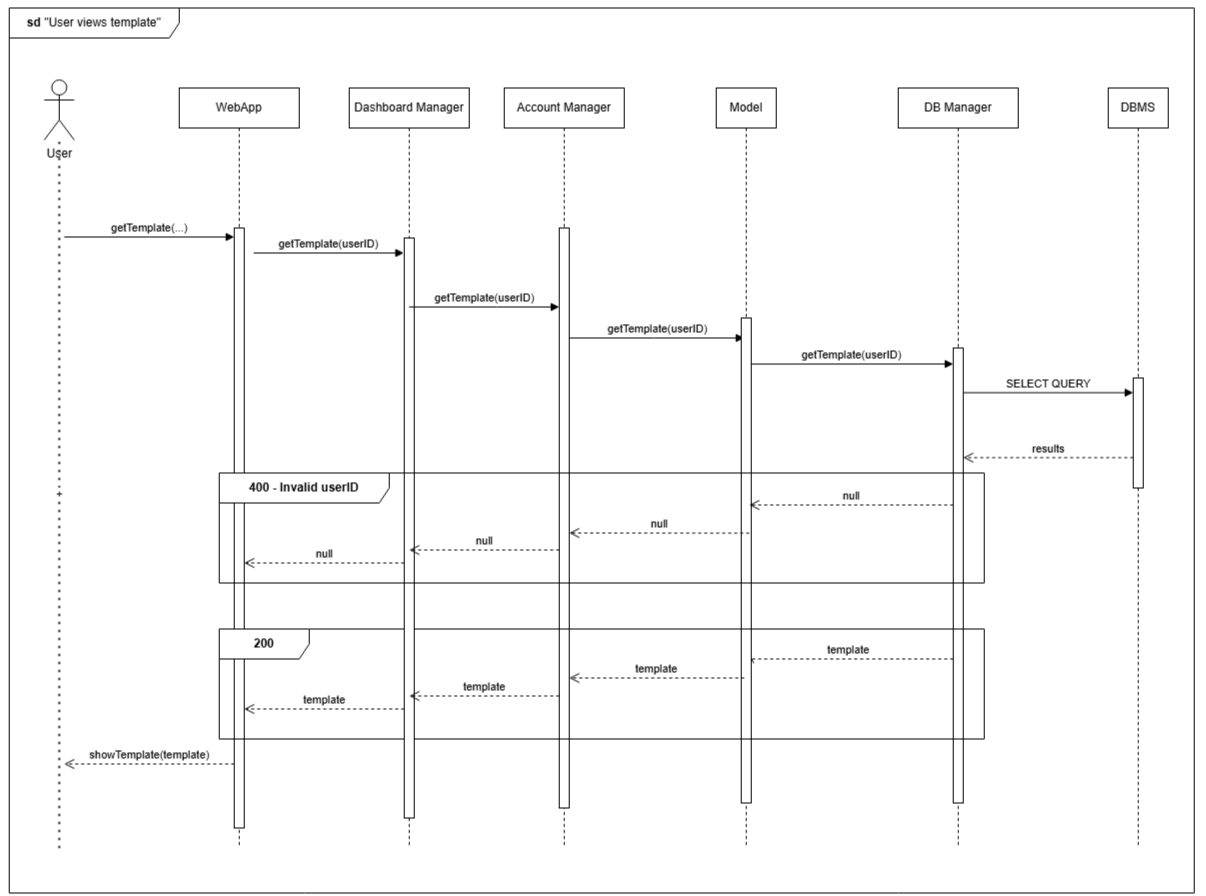
\includegraphics[scale = 0.5]{DD_figures/RuntimeView/UserViewsTemplateRV.png}\\
\caption{User Views Template}
\end{figure}
\newpage

\subsection{Component Interfaces}
\subsubsection{Authentication Manager}
\subsubsection*{AuthInterface}
User login(username:String, password:String)\\
bool register(info:UserInfo)

\subsubsection{Authentication Manager}
\subsubsection*{AuthInterface}
User login(username:String, password:String)\\
bool register(info:UserInfo)

\subsubsection{API Endpoints}
\subsection{Selected Architectural Styles and Patterns}
\subsection{Other Design Decisions}
\subsubsection{Scale-out}
\subsubsection{Relational Database}
\subsubsection{Token-Based Authentication and Authorization}
\subsubsection{Distributed MVC Pattern}

\section{User Interface Design}

\section{Requirements Traceability}

\begin{center}
    \begin{tabular}{|C{3cm}|p{10cm}|}
    \hline
    \multicolumn{2}{|c|}{\parbox{13cm}{R1: The system must allow a student who wants to register to sign up.}} \\
    \hline
    \centering C0 & DB Manager \\ 
    \hline
    \centering C3 & Authentication Manager \\ 
    \hline
    \centering C6 & Recommendation Manager \\ 
    \hline
    \centering C8 & Notification Manager \\ 
    \hline
    \centering C9 & Model \\ 
    \hline
    \centering C10 & Email Service Provider \\ 
    \hline
    \centering C11 & Notification Provider \\ 
    \hline
    \centering C13 & University Login Service \\ 
    \hline
    \end{tabular}
\end{center}

\begin{center}
    \begin{tabular}{|C{3cm}|p{10cm}|}
    \hline
    \multicolumn{2}{|c|}{\parbox{13cm}{R2: The system must allow a company who wants to register to sign up.}} \\
    \hline
    \centering C0 & DB Manager \\ 
    \hline
    \centering C3 & Authentication Manager \\ 
    \hline
    \centering C6 & Recommendation Manager \\ 
    \hline
    \centering C9 & Model \\ 
    \hline
    \centering C10 & Email Service Provider \\ 
    \hline
    \end{tabular}
\end{center}

\begin{center}
    \begin{tabular}{|C{3cm}|p{10cm}|}
    \hline
    \multicolumn{2}{|c|}{\parbox{13cm}{R3: The system must allow a university who wants to register to sign up.}} \\
    \hline
    \centering C0 & DB Manager \\ 
    \hline
    \centering C3 & Authentication Manager \\ 
    \hline
    \centering C8 & Notification Manager \\ 
    \hline
    \centering C9 & Model \\ 
    \hline
    \centering C10 & Email Service Provider \\ 
    \hline
    \centering C12 & National Education Dictionary API\\
    \hline
    \end{tabular}
\end{center}

\begin{center}
    \begin{tabular}{|C{3cm}|p{10cm}|}
    \hline
    \multicolumn{2}{|c|}{\parbox{13cm}{R4: The system must allow registered users to sign in using their credentials.}} \\
    \hline
    \centering C0 & DB Manager \\ 
    \hline
    \centering C1 & Dashboard Manager \\ 
    \hline
    \centering C2 & Account Manager \\ 
    \hline
    \centering C3 & Authentication Manager \\ 
    \hline
    \centering C9 & Model \\ 
    \hline
    \end{tabular}
\end{center}

\begin{center}
    \begin{tabular}{|C{3cm}|p{10cm}|}
    \hline
    \multicolumn{2}{|c|}{\parbox{13cm}{R6: The system must be able to send notifications to all users.}} \\
    \hline
    \centering C1 & Dashboard Manager \\ 
    \hline
    \centering C4 & Internship Manager \\ 
    \hline
    \centering C5 & Comment Manager \\ 
    \hline
    \centering C6 & Recommendation Manager \\ 
    \hline
    \centering C7 & Interaction Manager \\ 
    \hline
    \centering C8 & Notification Manager \\ 
    \hline
    \centering C10 & Email Service Provider \\ 
    \hline
    \centering C11 & Notification Provider \\ 
    \hline
    
    \end{tabular}
\end{center}

\begin{center}
    \begin{tabular}{|C{3cm}|p{10cm}|}
    \hline
    \multicolumn{2}{|c|}{\parbox{13cm}{R7: The system must allow registered students to upload their CVs on the platform.}} \\
    \hline
    \centering C0 & DB Manager \\ 
    \hline
    \centering C1 & Dashboard Manager \\ 
    \hline
    \centering C2 & Account Manager \\ 
    \hline
    \centering C6 & Recommendation Manager \\ 
    \hline
    \centering C8 & Notification Manager \\ 
    \hline
    \centering C9 & Model \\ 
    \hline
    \centering C11 & Notification Provider \\ 
    \hline
    \end{tabular}
\end{center}

\begin{center}
    \begin{tabular}{|C{3cm}|p{10cm}|}
    \hline
    \multicolumn{2}{|c|}{\parbox{13cm}{R8: The system must allow registered companies to post internship advertisements.}} \\
    \hline
    \centering C0 & DB Manager \\ 
    \hline
    \centering C1 & Dashboard Manager \\ 
    \hline
    \centering C4 & Internship Manager \\ 
    \hline
    \centering C6 & Recommendation Manager \\ 
    \hline
    \centering C8 & Notification Manager \\ 
    \hline
    \centering C9 & Model \\ 
    \hline
    \centering C11 & Notification Provider \\ 
    \hline
    \end{tabular}
\end{center}
\begin{center}
    \begin{tabular}{|C{3cm}|p{10cm}|}
    \hline
    \multicolumn{2}{|c|}{\parbox{13cm}{R9: The system must allow companies to review students' CVs and select candidates who meet their internship requirements.}} \\
    \hline
    \centering C0 & DB Manager \\ 
    \hline
    \centering C1 & Dashboard Manager \\ 
    \hline
    \centering C2 & Account Manager \\ 
    \hline
    \centering C9 & Model \\ 
    \hline
    \end{tabular}
\end{center}
\begin{center}
    \begin{tabular}{|C{3cm}|p{10cm}|}
    \hline
    \multicolumn{2}{|c|}{\parbox{13cm}{R10: The system must allow students to review internship advertisements and select them if they wish to apply.}} \\
    \hline
    \centering C0 & DB Manager \\ 
    \hline
    \centering C1 & Dashboard Manager \\ 
    \hline
    \centering C4 & Internship Manager \\ 
    \hline
    \centering C9 & Model \\ 
    \hline
    \end{tabular}
\end{center}
\begin{center}
    \begin{tabular}{|C{3cm}|p{10cm}|}
    \hline
    \multicolumn{2}{|c|}{\parbox{13cm}{R11: The system must allow students to manually search for internship opportunities and save them to their favorites.}} \\
    \hline
    \centering C0 & DB Manager \\ 
    \hline
    \centering C1 & Dashboard Manager \\ 
    \hline
    \centering C4 & Internship Manager \\ 
    \hline
    \centering C9 & Model \\ 
    \hline
    \end{tabular}
\end{center}
\begin{center}
    \begin{tabular}{|C{3cm}|p{10cm}|}
    \hline
    \multicolumn{2}{|c|}{\parbox{13cm}{R12: The system must notify students when there are updates regarding the internships they applied for or accepted.}} \\
    \hline
    \centering C0 & DB Manager \\ 
    \hline
    \centering C1 & Dashboard Manager \\ 
    \hline
    \centering C4 & Internship Manager \\ 
    \hline
    \centering C8 & Notification Manager \\ 
    \hline
    \centering C11 & Notification Provider \\ 
    \hline
    \end{tabular}
\end{center}
\begin{center}
    \begin{tabular}{|C{3cm}|p{10cm}|}
    \hline
    \multicolumn{2}{|c|}{\parbox{13cm}{R13: The system must notify a student and a company that accept each other.}} \\
    \hline
    \centering C0 & DB Manager \\ 
    \hline
    \centering C1 & Dashboard Manager \\ 
    \hline
    \centering C4 & Internship Manager \\ 
    \hline
    \centering C8 & Notification Manager \\ 
    \hline
    \centering C9 & Model \\ 
    \hline
    \centering C11 & Notification Provider \\ 
    \hline
    \end{tabular}
\end{center}\begin{center}
    \begin{tabular}{|C{3cm}|p{10cm}|}
    \hline
    \multicolumn{2}{|c|}{\parbox{13cm}{R14: The system must allow companies to choose a suitable date for the interview, but only after a match is done.}} \\
    \hline
    \centering C0 & DB Manager \\ 
    \hline
    \centering C1 & Dashboard Manager \\ 
    \hline
    \centering C4 & Internship Manager \\ 
    \hline
    \centering C8 & Notification Manager \\ 
    \hline
    \centering C9 & Model \\ 
    \hline
    \centering C11 & Notification Provider \\ 
    \hline
    \end{tabular}
\end{center}
\begin{center}
    \begin{tabular}{|C{3cm}|p{10cm}|}
    \hline
    \multicolumn{2}{|c|}{\parbox{13cm}{R15: The system must schedule an interview at the date and time specified by the company and notify the selected students.}} \\
    \hline
    \centering C0 & DB Manager \\ 
    \hline
    \centering C1 & Dashboard Manager \\ 
    \hline
    \centering C4 & Internship Manager \\ 
    \hline
    \centering C8 & Notification Manager \\ 
    \hline
    \centering C9 & Model \\ 
    \hline
    \centering C11 & Notification Provider \\ 
    \hline
    \end{tabular}
\end{center}

\begin{center}
    \begin{tabular}{|C{3cm}|p{10cm}|}
    \hline
    \multicolumn{2}{|c|}{\parbox{13cm}{R16: The system must recommend a student and an internship to each other if the student's profile matches the needs of the company.}} \\
    \hline
    \centering C0 & DB Manager \\ 
    \hline
    \centering C1 & Dashboard Manager \\ 
    \hline
    \centering C2 & Account Manager \\ 
    \hline
    \centering C4 & Internship Manager \\ 
    \hline
    \centering C6 & Recommendation Manager \\ 
    \hline
    \centering C8 & Notification Manager \\ 
    \hline
    \centering C9 & Model \\ 
    \hline
    \centering C11 & Notification Provider \\ 
    \hline
    \end{tabular}
\end{center}
\begin{center}
    \begin{tabular}{|C{3cm}|p{10cm}|}
    \hline
    \multicolumn{2}{|c|}{\parbox{13cm}{R17: The system must allow companies to offer internship proposals to selected students after the interview process is completed.}} \\
    \hline
    \centering C0 & DB Manager \\ 
    \hline
    \centering C1 & Dashboard Manager \\ 
    \hline
    \centering C4 & Internship Manager \\ 
    \hline
    \centering C8 & Notification Manager \\ 
    \hline
    \centering C9 & Model \\ 
    \hline
    \centering C11 & Notification Provider \\ 
    \hline
    \end{tabular}
\end{center}

\begin{center}
    \begin{tabular}{|C{3cm}|p{10cm}|}
    \hline
    \multicolumn{2}{|c|}{\parbox{13cm}{R18: The system must allow companies and students to give feedback at the end of the internship in which they took part.}} \\
    \hline
    \centering C0 & DB Manager \\ 
    \hline
    \centering C1 & Dashboard Manager \\ 
    \hline
    \centering C4 & Internship Manager \\ 
    \hline
    \centering C7 & Interaction Manager \\ 
    \hline
    \centering C8 & Notification Manager \\ 
    \hline
    \centering C9 & Model \\ 
    \hline
    \centering C11 & Notification Provider \\ 
    \hline
    \end{tabular}
\end{center}
\begin{center}
    \begin{tabular}{|C{3cm}|p{10cm}|}
    \hline
    \multicolumn{2}{|c|}{\parbox{13cm}{R19: The system must allow the student and company who got recommended to each other to give feedback about the recommendation.}} \\
    \hline
    \centering C0 & DB Manager \\ 
    \hline
    \centering C1 & Dashboard Manager \\ 
    \hline
    \centering C4 & Internship Manager \\ 
    \hline
    \centering C6 & Recommendation Manager \\ 
    \hline
    \centering C7 & Interaction Manager \\ 
    \hline
    \centering C8 & Notification Manager \\ 
    \hline
    \centering C9 & Model \\ 
    \hline
    \centering C11 & Notification Provider \\ 
    \hline
    \end{tabular}
\end{center}

\begin{center}
    \begin{tabular}{|C{3cm}|p{10cm}|}
    \hline
    \multicolumn{2}{|c|}{\parbox{13cm}{R20: The system must provide a suggested template to users for improving their CV or project description.}} \\
    \hline
    \centering C0 & DB Manager \\ 
    \hline
    \centering C1 & Dashboard Manager \\ 
    \hline
    \centering C2 & Account Manager \\ 
    \hline
    \centering C9 & Model \\ 
    \hline
    \end{tabular}
\end{center}

\begin{center}
    \begin{tabular}{|C{3cm}|p{10cm}|}
    \hline
    \multicolumn{2}{|c|}{\parbox{13cm}{R21: The system must notify students when there are updates regarding the results of the internships they have applied for.}} \\
    \hline
    \centering C0 & DB Manager \\ 
    \hline
    \centering C1 & Dashboard Manager \\ 
    \hline
    \centering C4 & Internship Manager \\ 
    \hline
    \centering C8 & Notification Manager \\ 
    \hline
    \centering C9 & Model \\ 
    \hline
    \centering C11 & Notification Provider \\ 
    \hline
    \end{tabular}
\end{center}

\begin{center}
    \begin{tabular}{|C{3cm}|p{10cm}|}
    \hline
    \multicolumn{2}{|c|}{\parbox{13cm}{R22: The system must allow selected students to accept or decline internship proposal sent by companies.}} \\
    \hline
    \centering C0 & DB Manager \\ 
    \hline
    \centering C1 & Dashboard Manager \\ 
    \hline
    \centering C4 & Internship Manager \\ 
    \hline
    \centering C8 & Notification Manager \\ 
    \hline
    \centering C9 & Model \\ 
    \hline
    \centering C11 & Notification Provider \\ 
    \hline
    \end{tabular}
\end{center}

\begin{center}
    \begin{tabular}{|C{3cm}|p{10cm}|}
    \hline
    \multicolumn{2}{|c|}{\parbox{13cm}{R24: The system must allow companies to view and manage applications for the internships they have posted.}} \\
    \hline
    \centering C0 & DB Manager \\ 
    \hline
    \centering C1 & Dashboard Manager \\ 
    \hline
    \centering C4 & Internship Manager \\ 
    \hline
    \centering C6 & Recommendation Manager \\ 
    \hline
    \centering C8 & Notification Manager \\ 
    \hline
    \centering C9 & Model \\ 
    \hline
    \centering C11 & Notification Provider \\ 
    \hline
    \end{tabular}
    
\end{center}
\begin{center}
    \begin{tabular}{|C{3cm}|p{10cm}|}
    \hline
    \multicolumn{2}{|c|}{\parbox{13cm}{R25: The system must allow students to view all details about the internships they have applied for, such as completion status, and deadlines.}} \\
    \hline
    \centering C0 & DB Manager \\ 
    \hline
    \centering C1 & Dashboard Manager \\ 
    \hline
    \centering C4 & Internship Manager \\ 
    \hline
    \centering C5 & Comment Manager \\ 
    \hline
    \centering C9 & Model \\ 
    \hline
    \end{tabular}
\end{center}

\begin{center}
    \begin{tabular}{|C{3cm}|p{10cm}|}
    \hline
    \multicolumn{2}{|c|}{\parbox{13cm}{R27: The system must allow universities to follow internship processes, handle complaints raised by students, and interrupt an internship if necessary.}} \\
    \hline
    \centering C0 & DB Manager \\ 
    \hline
    \centering C1 & Dashboard Manager \\ 
    \hline
    \centering C4 & Internship Manager \\ 
    \hline
    \centering C5 & Comment Manager \\ 
    \hline
    \centering C8 & Notification Manager \\ 
    \hline
    \centering C9 & Model \\ 
    \hline
    \centering C11 & Notification Provider \\ 
    \hline
    \end{tabular}
\end{center}

\section{Implementation, Integration and Testing Plan}
\subsection{Development Process and Approach}
\subsection{Implementation \& Integration Plan}
\subsubsection{Server Side}
\subsubsection{Client Side}
\subsubsection{Final Integration Test}
\subsection{Technologies}
\subsubsection{Development Technologies}
\subsubsection{Testing Technologies}

\section{Effort Spent}
\subsection{Effort Spent per Unit}

\section{References}
\subsection{References and Tools}

\end{document}
